\documentclass[11pt]{article}
%\usepackage[margin=1in]{geometry} 
\usepackage{template}

        

\usepackage[utf8]{inputenc} % allow utf-8 input
\usepackage[T1]{fontenc}    % use 8-bit T1 fonts
\usepackage{hyperref}       % hyperlinks
\usepackage{url}            % simple URL typesetting
\usepackage{booktabs}       % professional-quality tables
\usepackage{amsfonts}       % blackboard math symbols
\usepackage{nicefrac}       % compact symbols for 1/2, etc.
\usepackage{microtype}      % microtypography
\usepackage{lipsum}
\usepackage[labelfont=bf]{caption}
\usepackage{subcaption}
\usepackage{amsmath,amsthm,amssymb}
\usepackage[english]{babel}
\usepackage{comment}
\usepackage{enumitem}
\usepackage[ruled,vlined]{algorithm2e}
%\usepackage{algorithmic}
%\usepackage{algorithmicx}
\usepackage{gensymb}

\usepackage{graphicx}
\graphicspath{ {images/} }

\usepackage{floatrow}
\usepackage{listings}
\usepackage{minted}
\floatsetup[listing]{style=Plaintop}  


  
\newtheorem{theorem}{Theorem}[section]
\newtheorem{corollary}{Corollary}[theorem]
\newtheorem{lemma}[theorem]{Lemma}
\newtheorem{assumption}[theorem]{Assumption}
\newtheorem{definition}{Definition}[section]


\usepackage{float}
\usepackage{texments}
\usestyle{default} %other useful styles are, bw,  borland, vs
\usepackage[dvipsnames]{xcolor}
\usepackage[toc,page]{appendix}
%\usepackage[titletoc]{appendix}
\usepackage{minted}

\usepackage{chngcntr}
\counterwithin{figure}{section}
\counterwithin{table}{section}

%citation
\usepackage{epigraph}

\usepackage{graphicx}

\newcommand{\norm}[1]{\left\lVert#1\right\rVert}

\newcommand{\cac}[1]{{\textcolor{blue}[\textcolor{blue}{\bf{AC: }}{ \textcolor{blue}
              {#1}\textcolor{blue}]}}}
\newcommand{\cgv}[1]{{\textcolor{RedOrange}[\textcolor{RedOrange}{\bf{GV: }}{ \textcolor{RedOrange}
              {#1}\textcolor{RedOrange}]}}}

%\setcitestyle{square}

%%%%%%%%%%%%%%%%%%%%%%%%%%%%%%%%
%%      Tittle Page Start     %%
%%%%%%%%%%%%%%%%%%%%%%%%%%%%%%%%
\title{training a neural network with nonlinear conjugate gradient and limited-memory bfgs methods}
\author{
  Alessandro Cudazzo \\
  \texttt{alessandro@cudazzo.com} \\
  %% examples of more authors
   \And
  Giulia Volpi \\
  \texttt{giuliavolpi25.93@gmail.com} \\
  \AND
  Department of Computer Science, University of Pisa, Pisa, Italy
  %% Coauthor \\
  %% Affiliation \\
  %% Address \\
  %% \texttt{email} \\
  %% \And
  %% Coauthor \\
  %% Affiliation \\
  %% Address \\
  %% \texttt{email} \\
  %% \And
  %% Coauthor \\
  %% Affiliation \\
  %% Address \\
  %% \texttt{email} \\
}

%%%%%%%%%%%%%%%%%%%%%%%%%%%%%%%%
%%       Tittle Page End      %%
%%%%%%%%%%%%%%%%%%%%%%%%%%%%%%%%

\begin{document}

\maketitle
\begin{abstract}
Neural Networks are highly expressive models that have achieved the state of the art performance in many tasks as pattern recognition or natural language processing. Usually, stochastic momentum methods coupled with the classical Backpropagation algorithm for the gradient computation is used in training a neural network.
In recent years several methods have been developed to accelerate the learning convergence of first-order methods such as \textit{Classic Momentum}, also known as \textit{Polyak's heavy ball method} \cite{Polyak1964}, or the \textit{Nesterov} momentum \cite{10029946121}.
This work aims to go beyond the first-order methods and analyse some variants of the nonlinear conjugate gradient (NCG) and a specific case of limited-memory quasi-Newton class called L-BFGS as optimization methods. Them are combined with  the use of a line search that respects the strong Wolfe conditions to accelerate the learning processes of a feedforward neural network.  
\end{abstract}

\section{Introduction}


Over the years neural networks (NN) have been widely used in many areas, such as pattern recognition or image segmentation where they have overcome classic computer vision algorithms with the use of Convolution Neural Networks (CNN) \cite{DBLP:journals/corr/BadrinarayananK15} and very quickly became the state of the art in many other areas ( i.e. speech recognition, natural language processing, audio recognition all well illustrated in \cite{Goodfellow-et-al-2016}). 
As defined in \cite{Mitchell97}, a NN, as any other machine learning (ML) models, is said to learn from experience to some class of tasks if the performance, measured by a metric, improves with that experience.
Usually, the learning process that allows the improvement of the performance is related to an optimization algorithm where a quantity, called Error, is minimized/maximized: this is why the field of optimization is so central in machine learning. The optimization process can concern both the area of constrained optimization (i.e. in Support Vector Machine) or unconstrained (i.e in NN) and we will focus on the last one. With respect to neural networks and unconstrained optimization, the stochastic gradient descent (SGD) coupled with the back-propagation (BP) algorithms, for the gradient computation, remains a popular supervised learning algorithm to train a NN but is not the fastest in terms of convergence. 
The SGD is a first-order method and the convergence can be improved through the use of acceleration methods that are already well known in the classical literature of unconstrained optimization: \textit{Classic Momentum} also known as \textit{Polyak's heavy ball method} \cite{Polyak1964} or the \textit{Nesterov} momentum \cite{10029946121} developed respectively in 1960 e 1983. In \cite{sutskever2013} has been proved that the last two methods are very efficient in performing the training of a neural network without the use of second-order optimization methods. With this work, we want to go further beyond the classical first-order methods and investigate more complex methods that use high-order information during the training phase such as Nonlinear Conjugate Gradient and the L-BFGS from the class of Limited-Memory Quasi-Newton. Those methods lead to  a more accurate choice of the search direction and of the step size, by using information
from the second-order approximation. Even better, L-BFGS achieves super-linear convergence.

The remaining text is structured as follows. In Section~\ref{sec:NN}, we have summarised all the assumptions for neural networks seen as an unconstrained optimization problem. In section \ref{sec:NCG} and \ref{sec:QNM} the conjugate gradient and the limited-memory BFGS methods will be illustrated. The experiments are shown in Section~\ref{sec:experiment} and contains the results for three objective function derived from the MONKs dataset, while Section~\ref{sec:conclusions} is devoted to conclusions.



\section{The neural network}
\label{sec:NN}
The design of a Neural Networks model is biologically inspired by the brain and it's offer properties and capabilities \cite{Mitchell97,Goodfellow-et-al-2016, haykin2009neural}. This machine learning model has an elastic and adaptive ability, capable of learning from experience (the data provided) through a supervised process.  It can be considered as a network of interconnected units (artificial neurons) that adapt to perform a given task with the ability also to discover new knowledge. It can solve either a classification (binary/multi-class) or regression tasks. In this work, we will analyze a neural network from a mathematical point of view and a NN can be seen as a flexible function $h(\mathbf{x})$ that is a nested non-linear function:
\begin{equation}
    \label{eq:nn_function}
    h(\mathbf{x}) = f_k \left( \sum_{j}^J w_{kj} f_j \left( \sum_{i}^I w_{ji}x_i \right)\right) %= f_k \left( \sum_{j}^M w_{kj} f_j \left( net_j \right)\right) = f_k \left(net_k\right)
\end{equation}
where $h(\mathbf{x})$ is relative to a NN with one output neuron on the output layer, one hidden layer with J hidden neurons and input $\mathbf{x} \in \mathbb{R}^I$. Where $f_k$ is the activation function output neuron (linear or nonlinear function), $w_{kj}$ is a specific wights of the output neuron connected to the $j$-th hidden output neuron $f_j$ (a nonlinear activation function) that takes as input the linear combination of the products between $w_{ji}*x_i$.

So, the most important components of a NN are the nodes and architecture. Each node in the network will have associated a number of weights equal to the input of that node, a bias (which in our work will be included in the weights vector) and an activation function. The network can have different architectures with one or more hidden layers but the important thing is that each node in the hidden layers has a non-linear activation function (e.g. sigmoid). This allows the neural network to implement a linear basic expansion that is flexible and adaptive during the learning process thought the free parameters ($\mathbf{w}$) inside the non-linear activation function. Moreover, different architectures can lead to different hypothesis spaces that make the network more or less expressive for the task we are solving. This characterizes the neural networks by an important result which is the universal approximation theorem: an MLP network can approximate (arbitrarily well) every input-output mapping (provided enough units in the hidden layers). As concerns, the activation functions of neurons in the output layer can be either linear in case of a regression task or non-linear (e.g. sigmoid, softmax) in case of binary or multiclass classification tasks.

As in any other ML framework, we need a \emph{learning algorithm} that allows adapting the free-parameters of the model based on data provided in order to obtain the best approximation of the target function. This is often realized in terms of minimization of an error function on the training data set:
\begin{equation}
    \mathbf{w}^* = \min_{\mathbf{w} \;	\in \; \mathbb{R}^n} E(\mathbf{w})
    \label{eq:minimum}
\end{equation}
given a set of $l$ training examples $(\mathbf{x}_p,\mathbf{d}_p)$, where $\mathbf{x}_p \in \mathbb{R}^I$ and $\mathbf{d}_p \in \mathbb{R}^R$ we want to find the weights vector $\mathbf{w}^* = (w_1^*,w_2^*, ..., w_n^*) \in \mathbb{R}^n$  that minimize a Error fuction $E$ that measure the performace of a NN model on the training data.
\begin{equation}
E(\mathbf{w})  = \sum_{p=1}^{l}J(h(\mathbf{x}_p), \mathbf{d}_p)
\end{equation}
We can have different error function and the $J$ function defines the quantity to measure for each pattern. It is well known that in order to find a good model it is not only essential to minimize the error on the training set but that the model has to be able to generalize correctly concerning data not yet seen (e.g. on a validation set). We will analyze the optimization algorithms and their properties from a mathematical point of view, so it will be considered only a training set on how to perform the minimization. 

The optimization process is carried out using a classic iterative algorithm, chosen a starting point $\mathbf{w}_0$ up to a stop condition these steps are performed in an iterative manner:
\begin{enumerate}
    \item the function $h(\mathbf{x})$ is evaluated on the training set and then the error function is computed.
    \item the gradient is computed: $\nabla E(\mathbf{w})$.
    \item the weights are updated thought an update rule.
\end{enumerate}

For the discussion of the two main algorithms, the conjugate gradient and limited-memory BFGS, we need to define some information, on neural networks, that will be used later.

\subsection{Weights' initialization}
\label{sec:w_init}
The weights' initialization defines the starting point of the iterative algorithm. It is a very important phase and can lead to a better starting point and faster convergence. Many deep learning applications make use of a random weights initialization where each weight is drawn from a zero-mean Gaussian distribution $N(0,v^2)$ with a fixed standard deviation $v$ (e.g 0.01 in \cite{Krizhevsky_imagenetclassification}) or from an uniform distribution $U(-a,a)$ in the interval $(-a, a)$. Another technique, proposed by Glorot and Bengio in \cite{Glorot10understandingthe}, advice a properly scaled uniform distribution for initialization called \textbf{normalized initialization}:
$$ \mathbf{w} \sim U\left[-\frac{\sqrt{6}}{\sqrt{n + m}}, \frac{\sqrt{6}}{\sqrt{n + m}}\right]$$ 
where, $n$ and $m$ represent, respectively, the input and output size of a given layer. This initialization scheme is commonly referred to as the \textit{Xavier initialization}.

\subsection{Error function}
\label{sec:error_f}
To minimize an error function, we need to be able to compute the gradient so we must have a differentiable error function, differentiable activation functions and a network to follow the information flow. There are various types of error functions and for the analysis, we have decided to use the mean squared error (MSE) that measures the average of the squares of the errors overall examples, for both the classification and the regression tasks, namely:
\begin{equation}
\label{eq:error_function}
E(\mathbf{w})= \frac{1}{l} \sum_{p}^l \sum_{r}^R (\mathbf{d}_{pr}-h(\mathbf{x}_{pr}))^2  =   \sum_{p}^l E_p
\end{equation}
where $\mathbf{d}_{pr}$ is the actual output of a patter $p$ of the $r$-th output neuron, $R$ is the number of output neurons of the output layer and $l$ the total number of patterns in the training set.
%It should be noted that generally an error function is characterized by another component called regularization which allowing to control the complexity of the model. Our analysis will only include the minimization of the E without the regularization component.

The error function has the following properties:
\begin{itemize}
    \item It is bounded below in $\mathbb{R}^n$ by zero.
    \item By assuming to use only sigmoid activation functions on the hidden layer and linear or sigmoid activation functions on the output layer, we can say that since both are continuous and differentiable, E is a differentiable function. As sigmoid function we will use the logistic function defined as follow:
    $$ f(x) = \frac{1}{1+e^{-x}} \;,\; f^{'}(x) = f(x)(1 - f(x))$$
    \item The MSE is nonconvex function since is a composition of nonlinear activation function. It is characterized, by its nature, to be a nonconvex multimodal objective function that posses multi-local minima.
\end{itemize}

\subsection{The Backpropagation method for the gradient computation}
Now that we have a differentiable error function we can compute the gradient with the chain rule and the Backpropagation method.
$$\nabla E = - \frac{\partial E}{\partial \mathbf{w}} = - \frac{1}{l}\sum_{p}^l \frac{\partial E_p}{\partial \mathbf{w}} = \frac{1}{l} \sum_{p}^l \nabla_{p}\mathbf{w}$$
Where $ E = E(\mathbf{w})$ and $p$ refers to the $p$-th pattern in input the neural network. For the computation, let's consider for now only a network with 1 hidden and 1 output layers. 
\begin{figure}[H]
    \centering
    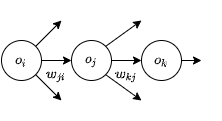
\includegraphics[scale = 0.6]{Images/flow_g.png}
    \caption{Network graph computation: $o_i$, $o_j$, $o_k$ are respectively the output of the  $i$-th input unit, $j$-th hidden unit and  $k$-th output unit. $w_{ji}$ is the weight associated with node $j$ connected to input $i$ (same for $w_{kj}$)}.
    \label{fig:computation_graph_backProp}
\end{figure}
\noindent The signal flow through the network in a forward direction as shown in Fig. \ref{fig:computation_graph_backProp} and a generic unit $t$ will compute the output $o_t$ with its activation function $f_t$ after computing the $net_t$:
\begin{equation}
\label{eq:generic_unit_eq}
    \left\{
        \begin{array}{ll}
            net_t = \sum_{q} w_{tq}o_q\\
            o_t = f_t(net_t)
        \end{array}
    \right.
\end{equation}
With Eq. \ref{eq:nn_function}, \ref{eq:error_function} and \ref{eq:generic_unit_eq} we can write the gradient respect a generic weights $d$ of unit $t$ assuming a pattern $p$:
$$\nabla_{p} w_{td} = - \frac{\partial E_{p}}{\partial w_{td}} = - \frac{\partial E_{p}}{\partial net_t} \cdot \frac{\partial net_t}{\partial w_{td}} = \delta_{t} \cdot o_d$$
Where, $\delta_t$ is the delta of unit $t$ and $o_d$ is the  input from a generic unit $d$ to the unit $t$, since
\[
 \frac{\partial net_t}{\partial w_{td}} = \frac{\partial \sum_{q} w_{tq}o_q}{\partial w_{td}} = o_d
\]

\noindent Now let's see the development of $\delta_t$:

$$\delta_t = - \frac{\partial E_p}{\partial net_t} = - \frac{\partial E_p}{\partial o_t} \cdot \frac{\partial o_t}{\partial net_t} = - \frac{\partial E_p}{\partial o_t} \cdot f'_t(net_t)$$
Where $- \frac{\partial E_p}{\partial o_t}$ changes according to the type of unit:

\begin{itemize}
    \item \textbf{Out unit K}
    $$- \frac{\partial E_p}{\partial o_k} = - \frac{\partial  \sum_{r}(d_{r}-o_{r})^2}{\partial o_{k}} = 2(d_{k}-o_{k})$$ 
    
    \item \textbf{Hidden unit J}
    $$- \frac{\partial E_p}{\partial o_j} = \sum_{k} - \frac{\partial E_p}{\partial net_k}\cdot \frac{\partial net_k}{\partial o_j} = \sum_{k} \delta_k \cdot w_{kj}$$ 
    \[
    \text{Since}\left\{
        \begin{array}{ll}
            - \frac{\partial E_p}{\partial net_k} = \delta_k \quad \text{(already computed)}\\
            \frac{\partial net_k}{\partial o_j} = \frac{\partial \sum_{z}^{}w_{kz}o_z}{\partial o_j} = w_{kj}
        \end{array}
    \right. 
\]

It expresses the variation of $E$ with respect to all the output unit $o_k$. Each $o_k$ (and $net_k$) depends on $o_j$, hence we introduce a sum over $k$.
\end{itemize}

\noindent \textbf{Summary}: We derived the gradient for a generic unit $t$ with input from $o_d$
$$ \nabla_p w_{ti} = \delta_t o_d$$
\begin{itemize}
    \item IF $t = k$ (output unit)
        \begin{equation}
            \label{eq:g_output_unit}
            \delta_k = 2(d_k - o_k)f_k^{'}(net_k)
        \end{equation}
    \item IF $t = j$ (hidden unit)
        \begin{equation}
            \label{eq:g_hidden_unit}
            \delta_j = \left( \sum_{k}^{}\delta_k w_{kj} \right) f_j^{'}(net_j)
        \end{equation}

\end{itemize}

\noindent This process can be generalised to $m$ hidden layers. Deltas come not only from the output layer but also from any up-layer to the considered layer in the computational graph. In other words, deltas flow from any units to which the considered unit is connected to and this is the reason why this process is called \textbf{Backpropagation}.

\subsection{Loss function: enforce Lipschitz continuity on the gradient}
\label{sec:l_lips_g}
From the analysis made it is clear that the neural network lives in a nonconvex domain and we have to solve a nonlinear unconstrained optimization problem. Some of the methods, that will be discussed in the next sections, require that the objective function gradient is global Lipschitz continuous for the convergence analysis. Looking at the result found in the backpropagation it is immediately clear that it is not possible to take this property into account. 
To better understand why this is not true, let's understand which functions are Lipschitz continuous if we consider the product and the linear combination of two Lipschitz continuous functions.\\

Lipschitz continuity is designed to measure change of function values versus change in the independent variable for a general function\footnote{In practical implementations, with the typical floating point numbers, instead: $f \;:\; I \rightarrow Q$ where I is a set of rational numbers.} $f \;:\; I \subseteq \mathbb{R}^n \rightarrow \mathbb{R}^m$:
\begin{theorem}
\label{th:l_sum}
Suppose that $f_1,..., f_n$ are Lipschitz continuous on $I$ with Lipschitz constants  $L_1 , ... , L_n$ respectively. Then the linear combination $c_1f_1 +...+c_nf_n$ is Lipschitz continuous on $I$ with Lipschitz constant $c_1L_1 +...+ c_nL_n$.
\end{theorem}
\noindent If we consider the product of two Lipschitz continuous functions on a bounded set $I$:
\begin{theorem}
\label{th:l_prodoct}
If $f_1(x)$ and $f_2(x)$ are Lipschitz continuous on a bounded set $I$ then $f_1(x)f_2(x)$ is Lipschitz continuous on I.
\end{theorem}
\noindent By analyzing the individual components of the gradient, we can see that it does not always respect the Th. \ref{th:l_sum} and \ref{th:l_prodoct}. This can be seen immediately by looking at Eq. \ref{eq:g_hidden_unit}, where the partial derivative is a composition of products of bounded Lipschitz continuous functions and the weights that are not restricted within a bounded set. In fact, in a iterative algortithm the gradient will be computed $k$ times until a stop condition is reached, the gradient Lipschitz continuity can be considered true only on the first iteration since the the weights are generated by a bounded and closed set, as seen in \ref{sec:w_init}, but not in any further iterations.\\

\noindent For the purpose of the analysis, instead of considering the error function $E$, we are going to consider as objective function, from now on, the loss function that is generally characterized by a further term,

\begin{equation}
    \label{eq:loss_f}
    L(\mathbf{w}) = E(\mathbf{w}) + \lambda\norm{\mathbf{w}}^2.
\end{equation}

%But if we consider an iterative optimization method that generate a monotonous decreasing sequence of values of the objective function and a regularization term added to the Error function we can enforce gradient Lipschitz continuity properties. From now on we will always use this new objective function, called Loss function,

Where $\lambda\norm{\mathbf{w}}^2$ is the regularization term and $\norm{\cdot}$ denotes the Euclidean norm. This new function is still bounded below in $\mathbf{R}^n$  by zero, differentiable and preserves all properties of $E$. Now, if we consider an iterative optimization method that generate a monotonous decreasing sequence of values of the objective function, as some of the methods that we will see (FR, PR+ and HS+ conjugate methods, and the L-BFGS), and $0<\lambda \leq 1$, we can derive
:

$$L(\mathbf{w}_i) \leq L(\mathbf{w}_0)\; , \; \forall i \in (1,2,3, ...k)$$
$$E(\mathbf{w}_i) + \lambda \norm{\mathbf{w}_i}^2 \leq L(\mathbf{w}_0)$$
Since, $E(\mathbf{w})$ is bounded below to zero,  $E(\mathbf{w}_i)$ is a constant and at least it will be zero, we can write that:
$$\lambda \norm{\mathbf{w}_i}^2 \leq L(\mathbf{w}_0)$$
$$\norm{\mathbf{w}_i}^2 \leq \frac{L(\mathbf{w}_0)}{\lambda} $$
$$\norm{\mathbf{w}_i} \leq \sqrt{\frac{L(\mathbf{w}_0)}{\lambda}} $$

we have thus proved that, in this case, the weights are bounded and the gradient is Lipschitz continuous. Moreover, weights live in a compact set because the set is closded too. \\

It is interesting to note that the regularization term is quite often used in the machine learning world and it allows to control the complexity of the model. Moreover, if the $\lambda$ constant is very low the weights will be subject to a very low or no regularization effect and they will be able to change arbitrarily (e.g. where a flexible model is needed it for a function approximation task). In this case, the error term will be the main part to be minimized to decrease the overall value of the loss, while still maintaining Lipschitz's continuous property on the gradient. Otherwise, with high $\lambda$ value the regularization term will be more important to minimise and it will lead to low weight and very rigid models.




\section{Nonlinear conjugate gradient method}
\label{sec:NCG}
To improve the performances of a Neural Network, instead of using the simple steepest-descent algorithm, an interesting second-order optimizer can be used: the \emph{Conjugate Gradient} method. It was proposed by Hestenes and Stiefel \cite{Hestenes1952} in 1952 and extended to nonlinear functions by Fletcher and Reeves \cite{Fletcher1964} in 1964. This optimizer is faster than the steepest-descent and ensures low-memory requirements. The methods generate a sequence of weights $\{ \mathbf{w}_k \}$, for every iteration of training $k$, using the iterative formula
\begin{equation}
\label{eq:ncg_updat_formula}
    \mathbf{w}_{k+1}=\mathbf{w}_k + \alpha_k \, \mathbf{d}_k, \,\,\, k=0,1,...,
\end{equation}
where $\alpha_k > 0$ is the step-length and $\mathbf{d}_k$ is a descent search direction. Hence the new weight update rule will be
\begin{equation}
    \Delta \mathbf{w}_k = \alpha_k \mathbf{d}_k.
\end{equation}

\noindent The search direction, also called the \emph{conjugate direction}, at the k-th iteration is defined by
\begin{equation}
\label{eq:ncg_direction}
    \mathbf{d_k} = 
    \begin{cases}
        -\mathbf{g}_k, & \text{if } k=0 \\
        -\mathbf{g}_k + \beta_k \,  \mathbf{d}_{k-1}, & \text{if } k>0, 
    \end{cases} 
\end{equation}
 where the \emph{conjugate gradient parameter} $\beta_k$ is a scalar that quantifies how much of the previous direction should be added to the new one, and $\mathbf{g}_k =\nabla L(\textbf{w}_k)$. Each new direction it's a linear combination of the steepest descent and the previous direction, hence the algorithm can compute a new vector $\mathbf{d}_k$ by only using the previous stored vector $\mathbf{d}_{k-1}$ and the current gradient $\mathbf{g}_k$. In fact, no operation with matrices are required compared to classical second-order methods and this is one of the main reasons why the algorithm is appealing for large optimization problem, as a neural networks optimization process, because allows to maintain the trade-off between rate of convergence, computational and storage cost. 
 
With regard to the conjugate gradient paramenter there are different formulas and each of them leads to different conjugate gradient methods with its computational efficiency and properties. The best-known formulas are called the Fletcher-Reeves (FR), Polak-Ribière (PR), and Hestenes-Stiefel (HS), and are given by 
\begin{equation}
  \beta_k^{FR} = \frac{\mathbf{g}_k^\mathsf{T} \, \mathbf{g}_k}{\mathbf{g}_{k-1}^\mathsf{T} \, \mathbf{g}_{k-1}},  
\end{equation}
\begin{equation}
  \beta_k^{PR} = \frac{\mathbf{g}_k^\mathsf{T} \, (\mathbf{g}_k - \mathbf{g}_{k-1})}{\|\mathbf{g}_{k-1}\|^2},  
\end{equation}
\begin{equation}
  \beta_k^{HS} = \frac{\mathbf{g}_k^\mathsf{T} \, (\mathbf{g}_k - \mathbf{g}_{k-1})}{(\mathbf{g}_k - \mathbf{g}_{k-1})^\mathsf{T} \, \mathbf{d}_{k-1}}.  
\end{equation}
Now, in order to make complete the whole algorithm, after computing $\mathbf{d}_k$, the step-length $\alpha_k > 0$ has to be found. In order to do that we need to pay some attention about the line search used to choice the alpha. When dealing with strongly convex quadratic functions and \emph{exact line search}, namely,
\begin{equation}
    \label{eq:exact_linesearch}
    \alpha_k = \text{arg}\min\limits_{\alpha} \,\{ L(\mathbf{w}_k + \alpha \mathbf{d}_k); \; \alpha > 0 \},
\end{equation}
that compute the exact minimizer, the algorithm reduces to the linear conjugate gradient method and this ensures that each direction is a descent direction \cite{Nocedal} for all the methods. But we are dealing with a non-linear case and the direction $\mathbf{d}_k$ not always hold the condition to be a descent direction unless certain conditions are satisfied, so we have to ensure that $\mathbf{d}_k$ has a descent property, namely, 
\begin{equation}
    \mathbf{g}_k^T \mathbf{d}_k \;< \;0.
\end{equation}
Let's consider the Fletcher-Reeves method for now, the inner product between Eq.~\ref{eq:ncg_direction} and the gradient $\mathbf{g}_k$ will tells us that at the first iteration we will have a descent direction by construction and for others we have to analyse
\begin{equation}
\label{eq:descent_dir_property}
    \mathbf{g}_k^T\mathbf{d}_k = - \norm{\mathbf{g}_k}^2 + \beta^{FR}_k\mathbf{g}^T_k \mathbf{d}_{k-1}.
\end{equation}
Thus if the the line search is exact, we have $\mathbf{g}^T_k \mathbf{d}_{k-1} = 0$ becouse the $\alpha_{k-1}$ is a local minimizer of our objective function along the direction $\mathbf{d}_{k-1}$. Consequently, this case led to a descent direction. Since the exact line search is usually expensive and impractical, a \emph{inexact line search} is often consider in the implementation of non-linear conjugate gradient methods. However, when the line search is not exact, the second term in Eq. \ref{eq:descent_dir_property} may dominate the first term and the descent property may not be true. A simple restart with $\mathbf{d}_k = -\mathbf{g}_k$ might help to avoid this situation, but will probably degrade the numerical performance since the previous direction $\mathbf{d}_k$ is discarded \cite{Powell1977}. However if we consider an inexact line-search with strong Wolfe conditions, which are,

    \begin{equation}
    \label{eq:wolfe1}
        L(\mathbf{w}_k + \alpha \, \mathbf{d}_k) \, \leq \, L(\mathbf{w}_k)\, + \, c_1 \, \alpha \, \mathbf{g}_k^\mathsf{T} \, \mathbf{d}_k,
    \end{equation}
    \begin{equation}
    \label{eq:wolfe2}
        |\mathbf{g}(\mathbf{w}_k + \alpha \, \mathbf{d}_k)^\mathsf{T} \mathbf{d}_k|\, \leq  \, - c_2 \, \mathbf{g}_k^\mathsf{T} \, \mathbf{d}_k,
    \end{equation}

with $0 < c_1 < c_2 < \frac{1}{2}$ (in place of the classical condition $c_2 < 1$ \cite{Nocedal} as shown in Sec.~\ref{sec:ncg_line_search}) condition \ref{eq:wolfe2} implies that Eq. \ref{eq:descent_dir_property} is negative (see Sec~\ref{sec:ncg_global_convergence}). With regard to other methods (PR, HS) strong Wolfe conditions do not guarantee that $\mathbf{d}_k$ is always a descent direction. Nevertheless, Powell \cite{powell} showed that the PR method cycles without obtaining the solution, with an exact line search, same can be shown for HS since they are identical with an exact line search $\mathbf{g}^T_k \mathbf{d}_{k-1} = 0$.
To overcome this problem, as suggested by Powell \cite{powell}, those methods must be modified in
\begin{equation}
\label{eq:beta_modified}
  \beta^+ = max\{\beta, \, 0\}.  
\end{equation}
Then a simple adaptation of the strong Wolfe conditions ensures that the descent property holds and, from now on, we will refer to them as PR+ and HS+. This modification introduces a sort of restart of the algorithm, in case the $\beta$ found is negative. Indeed the algorithm puts aside the last search direction and restarts with the steepest descent.

We can finally put everything together and define the whole algorithm in Algo~\ref{alg:conjugate}.

\begin{algorithm}[H]
%\footnotesize
\label{alg:conjugate}
\SetAlgoLined
 \textbf{init}: starting point $\mathbf{w}_0$, $max\_iter$, $\varepsilon = 10^{-4}$, $k = 0$\;
 \While{k < max\_iter}{
  Evaluate the Loss function $L_k$ and its gradient $g_k$\;
  \If{$\norm{g_k} < \varepsilon$}{\textbf{return} Loss $L_k$}
  Compute $\beta_k$ with one of the methods PR, FR, HS\;
  Compute the descent direction $\mathbf{d}_k$ by \emph{conjugate direction}\;
  Compute the step-legnth $\alpha_k$ with a Line Search satisfying the Strong Wolfe conditions\;
  Update the weights $\mathbf{w}_{k+1} \leftarrow \mathbf{w}_k + \alpha_k \,\mathbf{d}_k$\;
  Set $k \leftarrow k + 1$\;
 }
 \caption{Nonlinear Conjugate Gradient}
\end{algorithm}
\vspace{+6pt}
Several beta formulas have been presented and each of them requires a different theoretical analysis. As discussed in \cite{nocedal_global_convergence} the Fletcher-Reeves \cite{Fletcher1964} method can be as efficient as the Polak-Ribire and Hestenes Stiefel methods, but it is often much slower and erratic. Moreover, as shown by Powell \cite{Powell1977}, the Fletcher-Reeves, under some circumstances, can produce very small displacements and it needs some restart along the gradient direction in order to recover. Despite these drawbacks, Zoutendijk
\cite{zoutendijk1970northholland} has shown that the method cannot fail. He proved that the Fletcher-Reeves
method with exact line searches is globally convergent on general functions and Al-Baali \cite{baali} extended this result to inexact line searches.
The Polak-Ribire and Hestenes-Stiefel methods tend to be more robust and efficient. They are to be preferred over the Fletcher-Reeves method. They are very similar in term of theoretical convergence properties too, in fact, as we've already said, they need to restart, since the direction can fail to be a descent direction~\cite{Nocedal,Powell1977}. So Polak-Ribire and Hestenes-Stiefel are not featured by having a global convergence result without restart.
All this makes those methods attractive to be studied in our case. Thus, we will try to observe how these behaviours can affect our neural network objective function optimization process used in the experimental phase.\\

A strong Wolfe inexact line search was implemented for our experiments, this will be explained extensively in the next subsection. Having defined this we will focus on the convergence analysis of the algorithm in our specific case and finally conclude with the convergence rate analysis.


\begin{comment}
One thing in common to these formulas, they must guarantee the global convergence of the method. Al-Baali \cite{baali} proved that the FR method with inexact line searches is globally convergent on general functions. Moreover, he showed that using strong Wolfe conditions always generates descent directions.  Instead, for the PR and HS method, the strong Wolfe conditions by themselves do not guarantee that $\textbf{d}_k$ is always a descent direction. So, when the function to be minimized is convex and quadratic, there are no problems and the Conjugate Gradient algorithm ensures the convergence in \emph{n} steps, however, when dealing with nonquadratic functions, like in this case, the direction computed could be not a descent direction. To overcome this issue, all the methods must be modified in
\begin{equation}\label{eq:beta_modified}
  \beta = max\{\beta, \, 0\},  
\end{equation}
to ensure global convergence. This modification introduces a sort of \emph{restart} of the algorithm, in case the $\beta$ found is negative. Indeed the algorithm puts aside the last search direction and restarts with the steepest descent.
\end{comment}

\subsection{Strong Wolfe inexact line search}
\label{sec:ncg_line_search}
\begin{comment}
After the computation of the new direction $\mathbf{d}_k$, the step-length $\alpha_k > 0$ has to be found. The step-length is a simple scalar that, in the linear version of the method, was computed with a formula. However, in the nonlinear variant of the Conjugate Gradient, a line search has to be performed to find the right step size, which minimizes the Loss ($L$) function along $\mathbf{d}_k$.
\begin{equation}\label{linesearch}
    \alpha_k = \min\limits_{\alpha} \,\, L(\mathbf{w}_k + \alpha \mathbf{d}_k).
\end{equation}
We could perform a \emph{exact line search} and find the best $\alpha$ as the global minimizer of Eq.(\ref{linesearch}), but this would take too much time. Even searching for a local minimizer would bee too expensive. Hence, the smarter way is to perform an \emph{inexact line search}, that tries out a sequence of candidate values for $\alpha$ and accepts the first one satisfying some conditions. In this way, we can obtain a relevant reduction of the Loss at a minimal cost.\\
\end{comment}
For our implementation, we decided for a line search that satisfies the strong Wolfe conditions. This line search is done in two stages: a \emph{bracketing phase}, that finds an interval containing step lengths that minimize the Loss and an \emph{interpolation phase} that, given the interval, finds an acceptable step length. Strong Wolfe condition have already been introduced in Eq.~\ref{eq:wolfe1} and \ref{eq:wolfe2}. Here, we will discuss their behaviour in detail.
\begin{itemize}
    \item \emph{Armijo} condition Eq.~\ref{eq:wolfe1} is the \emph{sufficient decrease} condition
    where $c_1 \in (0,1)$ is a constant and  $\mathbf{g}_k^\mathsf{T}\mathbf{d}_k$ is the directional derivative. It ensures that the step-length $\alpha$ is not too large and forces a sufficient decrease in the function. However, not sufficient to guarantee convergence, because it is satisfied for all sufficiently small values of $\alpha >0$. The constant $c_1$ has to be quite small in general.  
    
    \item \emph{Strong Wolfe} condition Eq.~\ref{eq:wolfe2}
    where $c_2 \in (c_1,1)$ is a constant. This condition ensures that the slope of the function after moved by a step $\alpha$ (that is not too small because of this condition) along the direction $\mathbf{d}$ is greater than $c_2$ times the initial slope. Moreover, the strong condition doesn't allow the derivative $\mathbf{g}(\mathbf{w}_k + \alpha \, \mathbf{d}_k)^\mathsf{T} \mathbf{d}_k$ to be too positive and ensures that $\alpha$ is close to a minimizer of the function.
\end{itemize}

In our experimental setting, as suggested in~\cite{Nocedal}, we used $c_1 = 10^{-4}$ and $c_2 = 0.1$ and our strong Wolfe line search follows the one described in \cite{Nocedal} and is composed by two functions: \verb|line_search| and \verb|zoom|. They are both illustrated in Algo. \ref{algo:line_search} and \ref{algo:zoom} where it is assumed that: $\phi(\alpha) = L(\mathbf{w}_k + \alpha \mathbf{d}_k)$ and $\mathbf{d} = \mathbf{d}_k$. 

\begin{algorithm}
%\footnotesize
\SetAlgoLined
 \textbf{init}: $\alpha_0 \leftarrow 0$, choose $\alpha_{max} > 0$ and $\alpha_1 \in (0, \, \alpha_{max})$\;
 $i \leftarrow 1$\;
 \While{i < max\_iter}{
  Evaluate $\phi(\alpha_i)$\;
  \If{$[\phi(\alpha_i) > \phi(0) \, + \, c_1 \, \alpha_i \, \nabla \phi(0)^\mathsf{T}d] \,\, or \,\, [\phi(\alpha_i) \leq \phi(\alpha_{i-1}) \,\, and \,\, i > 1]$}{
  $\alpha_* \leftarrow \mathbf{zoom}(\alpha_{i-1}, \, \alpha_i)$\;
  \textbf{return} $\alpha_*$\;
  }
  Evaluate $\nabla \phi(\alpha_i)^\mathsf{T}d$\;
  \If{$|\nabla \phi(\alpha_i)^\mathsf{T}d| \leq -c_2 \, \nabla \phi(0)^\mathsf{T}d$}{
  $\alpha_* \leftarrow \alpha_i$\;
  \textbf{return} $\alpha_*$\;
  }
  \If{$\nabla \phi(\alpha_i)^\mathsf{T}d \geq 0$}{
  $\alpha_* \leftarrow \mathbf{zoom}(\alpha_i, \, \alpha_{i-1})$\;
  \textbf{return} $\alpha_*$\;
  }
  Choose $\alpha_{i+1} \in (\alpha_i, \, \alpha_{max})$\;
  $i \leftarrow i + 1$\;
 }
 \caption{Line Search}
 \label{algo:line_search}

\end{algorithm}

\begin{algorithm}
%\footnotesize
\SetAlgoLined
 \While{i < max\_iter}{
  $\alpha_j \leftarrow quadratic\_cubic\_interpolation(\alpha_{lo}, \, \alpha_{hi})$\;
  Evaluate $\phi(\alpha_j)$\;
  \eIf{$[\phi(\alpha_j) > \phi(0)\, +\, c_1 \, \alpha_j \, \nabla \phi(0)^\mathsf{T} \, d_0]\,\, or \,\,[\phi(\alpha_j) \leq \phi(\alpha_{lo})]$}{
  $\alpha_* \leftarrow \alpha_j$\;
  \textbf{return} $\alpha_*$\;
  }{
  Evaluate $\nabla \phi(\alpha_j)^\mathsf{T}d$\;
  \If{$|\nabla \phi(\alpha_j)^\mathsf{T} d|\leq - c_2 \, \nabla \, \phi(0)^\mathsf{T} \, d$}{
  $\alpha_* \leftarrow \alpha_j$\;
  \textbf{return} $\alpha_*$\;}
  \If{$\nabla \phi(\alpha_j)^\mathsf{T}d\,(\alpha_{hi} - \alpha_{lo}) \geq 0$}{
  $\alpha_{hi} \leftarrow \alpha_{lo}$\;}
  }
  Set $\alpha_{lo} \leftarrow \alpha_j$\;
  $i \leftarrow i + 1$\;
 }
 \caption{zoom}
 \label{algo:zoom}

\end{algorithm}

\subsection{Convergence analysis}
\label{sec:ncg_global_convergence}
Now we are going to understand which method is globally convergent and what is needed to ensure this property for each nonlinear conjugate gradient method using a practical line search. Finally, we will conclude with the same analysis but by considering our loss function defined in Eq.~\ref{eq:loss_f}.

Let's consider, once again, first the analysis for FR method. First, we have to consolidate what has been said about the descent direction when an inexact line-search is used to compute the step-length.\\

\noindent For the purposes of this section, we need the following assumptions on the objective function.
\begin{assumption}
\label{as:1}
The level set $\mathcal{L} = \{ \mathbf{w}\, | \, L(\mathbf{w}) \leq L(\mathbf{w}_0)\}$ is bounded, namely, there exists a constant $B > 0$ such that:
$$ \norm{\mathbf{w}} \leq B, \; \forall i \in \mathcal{L}$$ 
\end{assumption}
\begin{assumption}
\label{as:2}
    In some neighborhood $\mathcal{N}$ of $\mathcal{L}$, the objective function L is continuously differentiable, and its gradient is Lipschitz continuous, there exists a constant $C > 0$ such that 
    $$
      \|\mathbf{g}(\textbf{w}) - \mathbf{g}(\tilde{\textbf{w}})\| \, \leq \,  C \| \mathbf{w} - \tilde{\mathbf{w}}\|,\; \forall \mathbf{w}, \tilde{\mathbf{w}} \in \mathcal{N}
    $$
    It follows directly from A.~\ref{as:1} and A.~\ref{as:2} that there exists a positive constant $\gamma>0$ such that:
    $$\norm{\mathbf{g}(\textbf{w})} \, \leq\, \gamma, \;\; \forall \mathbf{w} \in \mathcal{L} $$
\end{assumption}
Under assumptions (\ref{as:1},\ref{as:2}) we can state the following Lemma.
\begin{lemma}
\label{lemma:descent_dir}
Suppose that Algorithm~\ref{alg:conjugate} is implemented with a step length $\alpha_k$ that satisfies the strong
Wolfe conditions (\ref{eq:wolfe1},\ref{eq:wolfe2}) with $0 < c_1 < c_2 < \frac{1}{2}$ . Then the method generates descent directions $\mathbf{d}_k$
that satisfy the following inequalities:
\begin{equation}
    -\frac{1}{1-c_2} \leq \frac{\mathbf{g}_k^T\mathbf{d}_k}{\norm{\mathbf{g}_k}^2} \leq \frac{2c_2 - 1}{1 -c_2},\; \; \text{for all $k = 0,1, ....$}
\label{eq:lemma_descent_dir}
\end{equation}
\end{lemma}
This Lemma, well proved in~\cite{Nocedal}, tells us that we have a descent direction\\
%Moreover can be used to show, easly, the weakness which we discussed.





Then, the Zoutendijk's theorem will be our main tool and is defined as follows.

\begin{theorem}[Zoutendijk’s theorem]
\label{th:Zoutendijk}
Consider any iteration of the form (\ref{eq:ncg_updat_formula}), where $\mathbf{d}_k$ is a descent direction and $\alpha_k$ satisfies the Wolfe conditions (\ref{eq:wolfe1},\ref{eq:wolfe2}). Suppose that Assumptions \ref{as:1} and \ref{as:2} hold, then
\begin{equation}
    \sum_{k > 0 } \cos^2 \theta_k \norm{\mathbf{g}_k}^2 \, < \, 0
    \label{eq:Zoutendijk_condition}
\end{equation}
\end{theorem}
This theorem is proved and well explained in~\cite{Nocedal, nocedal_global_convergence}. By combining Zoutendijk's result and Lemma \ref{lemma:descent_dir}, Al-Baali~\cite{baali} has proved that the FR method is globally convergent with the following theorem.

\begin{theorem}[Al-Baali \cite{baali}]
\label{th:FR_convergence}
If Assumptions \ref{as:1} and \ref{as:2} hold, and that Algorithm \ref{alg:conjugate} is implemented with a line search that satisfies the strong Wolfe conditions, with $0 < c_1 < c_2 < \frac{1}{2}$ in order to have a descent direction. Then
\begin{equation}
      \lim_{k\to\infty} \mathrm{inf} \, \|\mathbf{g}_k\| = 0.
\end{equation}
\end{theorem}

Instead, PR and HS methods do not always guarantee a descent direction so, the same global convergence result, as for FR, cannot be achieved. Gilbert and Nocedal have studied the global convergence for nonnegative $\beta_k$ (see \cite{nocedal_global_convergence}) and the following theorem proves that those method are globally convergent.
\begin{theorem}
\label{th:beta_mod_conv}
If Assumptions \ref{as:1} and \ref{as:2} hold, the Algorithm \ref{alg:conjugate} is implemented with a line search that satisfies the strong Wolfe conditions in order to have a descent direction and $\beta_k \geq 0$ for all $k$. Then
\begin{equation}
      \liminf_{k\to\infty} \, \|\mathbf{g}_k\| = 0.
\end{equation}
\end{theorem}

Therefore, the global convergence property can be proved too for the modified $\beta_k$ in Eq. \ref{eq:beta_modified} (PR+ and HS+) suggested by Powell \cite{powell}.\\


It seems that FR is characterised by some very fascinating theoretical convergence properties when compared to methods such as PR and HS, unless restart is used. However, from a practical point of view, there are some observations to be taken into account. We have already mentioned that FR can be subject to produce very small displacements, in fact, this is can be consider the main weakness of this method. We will argue that if the method generate a very small step or a bad direction, then this behaviour can continue for a very large number of iteration unless a restart is made. Initially observed by Powell~\cite{powell} with an exact line search, this can be proved too for an inexact line searches as showed by Nocedal~\cite{nocedal_global_convergence} using Lemma \ref{lemma:descent_dir}. We will state here what Nocedal has proven and in order to show this behaviour, let's define $\theta_k$ as the angle between $\mathbf{d}_k$ and the steepest descent direction $-\mathbf{g}_k$, namely,
\begin{equation}
    \label{eq:cos_theta}
    \cos \theta_k = \frac{-\mathbf{g}_k^T \mathbf{d}_k}{\norm{\mathbf{g}_k}\norm{\mathbf{d}_k}},
\end{equation}
and suppose that at iteration $k$ a bad search direction is generated, such that $\cos \theta_k \approx 0$ given by an angle of nearly 90\degree of $\mathbf{d}_k$ with $\mathbf{g}_k$. By using Eq.~\ref{eq:cos_theta} and multiplying both side of Eq. \ref{eq:descent_dir_property} by $ \norm{\mathbf{g}_k} / \norm{\mathbf{d}_k}$, we get as a result
\begin{equation}
    -\frac{1-2c_2}{1-c_2}\frac{\norm{\mathbf{g}_k}}{\norm{\mathbf{d}_k}} \leq \cos \theta_k \leq \frac{1}{1 -c_2} \frac{\norm{\mathbf{g}_k}}{\norm{\mathbf{d}_k}},\; \; \text{for all $k = 0,1, ....$}
\end{equation}
then, $\cos \theta_k \approx 0$ if and only if
$$ \norm{\mathbf{g}_k} \ll \norm{\mathbf{d}_k}.$$
This means that $\mathbf{w}_{k+1} \approx \mathbf{w}_k$, therefore $\mathbf{g}_{k+1} \approx \mathbf{g}_k$ and
$$ \beta^{FR}_{k+1} \approx 1.$$
By using all this approximation we will have that $\norm{\mathbf{g}_{k+1}} \approx \norm{\mathbf{g}_k} \ll \mathbf{d}_k$ and we can conclude that
$$ \mathbf{d}_{k+1} \approx \mathbf{d}_k.$$
It's clear that a bad move led to a long sequence of bad moves and the only way to avoid this is to restart with steepest descent direction at some point. Nocedal~\cite{nocedal_global_convergence} showed a practical example where, this undesirable behavior, can be observed in practice, moreover in that example the FR method performs much better if it is periodically restarted along the steepest descent direction in order to avoid the cycle of bad moves. This is why the FR method is highly recommended to implement it with a kind of restart strategy. On the other hand, the other methods (PR, HS, PR+, HS+) would behave quite differently in this situation. As we have already said, all of them behave identically to FR method in the quadratic case but the definition differs
in nonlinear case and, in particular, when there is stagnation if $\mathbf{g}_{k+1} \approx \mathbf{g}_k$ then those methods will have $\beta^+ \approx 0$ given an automatic restart and that why they tend to be more robust and efficient. Clearly restart is very important in the implementation of the conjugate algorithm for different purposes, avoid weakness (in the FR) or avoid negative directions of PR and HS in order to reach global convergent properties (PR+ and HS+). Anyway, the methods' behaviour could lead to different efficiency results depending on the problem being solved. So, given the global convergence results, the pros and cons found for each method, we will be compare them in our specific case in the experimental section to understand which one works best in the case of a nonlinear function derived from a neural network.\\


To conclude, let's analyze each method in our specific case. First, we focus in the case where the Loss function (see Eq.~\ref{eq:loss_f}) has $0<\lambda \leq 1$. We are able to prove that the FR method will converge to a stationary point with Th.~\ref{th:FR_convergence} because a descent direction is always taken if a strong Wolfe line search with $0 < c_1 < c_2 < \frac{1}{2}$ is used in the Algo.~\ref{alg:conjugate}, assumptions \ref{as:1} and \ref{as:2} always hold. Those assumptions are satisfied because, as it has been proved in Sec.~\ref{sec:l_lips_g}, due to the monotonic property of the FR method and the regularization term, the level set is bounded and, as a direct consequence, given the composition of the gradient, the gradient of the loss function is Lipschitz continuous. Anyway, attention must be paid to the main weakness of the FR method indicated in the analysis. Instead, we are not able to prove that PR and HS method will converge to a stationary point because a descent direction is not always guarantee and, because of this, Th.~\ref{th:FR_convergence} does not hold and the assumptions required (A. \ref{as:1}, \ref{as:2}) cannot be proved with the analysis in Sec.~\ref{sec:l_lips_g} due to the absence of the monotonic properties in these methods. As regards the PR+ and HS+,  Th.~\ref{th:beta_mod_conv} proves that we have the convergence to a stationary point because a descent direction is always ensured through the restart of the modified method (see Eq.~\ref{eq:beta_modified}) and all the remaining assumptions of the theorem can be proved as for the FR method. On the other hand, if we consider the case where the $L$ function has $\lambda = 0$ we cannot prove the convergence property to any of the described methods because the analysis made in Sec.~\ref{sec:l_lips_g} can't be applied and assumptions \ref{as:1} and \ref{as:2} will not hold.\\


%\cac{placeholder: concludere così o agganciarsi alle osservazioni dell'analisi sperimentale a fine report}

\begin{comment}
So, if we use $\beta$ modified as in Eq. \ref{eq:beta_modified}, and a Line Search as described in \ref{alpha} to find $\alpha_k$, then, how explained by Gilbert and Nocedal in \cite{nocedal_global_convergence}, the global convergence of the algorithm hold. Hence we have
\begin{equation}
      \lim_{k\to\infty} \mathrm{inf} \, \|\mathbf{g}_k\| = 0.
\end{equation}
\end{comment}

\subsection{Convergence rate analysis}
For what concerns the convergence rate analysis, most of the theory of conjugate gradient methods assume that the line search is exact. It has been hypothesised that the conjugate gradient method for minimizing functions of several variables has a superlinear rate of convergence, but it was later proved that this hypothesis was false. In fact, the first result on this subject has been reported by Crowder and Wolfe \cite{Crowder_rate} where they showed that the rate of convergence is linear and, by constructing an example, that Q-superlinear convergence is not achievable. Then, Powell~\cite{powell_rate_conv} has taken into account the analysis of a quadratic function with $n$ variables.
The quadratic case is very interesting since an iterative algorithm should be able to manage it efficiently. Moreover, if we consider a general differentiable function and if the minimization algorithm is taking small steps, then we can say that it enters a region where the objective function is quadratic. The follow stronger result has been proved by Powell. 

\begin{theorem}
If the conjugate gradient algorithm is applied to a quadratic function or enters a region where the objective function is quadratic,
then either termination is obtained within $(n + 1)$ iterations or convergence to the solution occurs at a linear rate.
\end{theorem}

But conjugate gradient methods are used to minimize general function too (nonlinear, nonquadratic, functions on $\mathbb{R}^n$). Cohen in \cite{Cohen_rate_conv} has proven that restarting leads to n-step quadratic convergence of the methods for general objective functions. We will state here the main result of its work.
\begin{theorem}
\label{th:cohen_rate_cg}
    Suppose the conjugate gradient algorithm (PR) or (FR) is used to solve the Minimum Problem (Eq. \ref{eq:minimum}) where we reinitialize the conjugate variable $\beta$ every $r$ steps (where $r \geq n$). Let $\mathbf{w}_0, \,\mathbf{w}_1, \,\mathbf{w}_2,\, .\, .\, .\,$ be the sequence formed; then there exists a constant $C$ that
    \begin{equation}
     \limsup\limits_{k\,\rightarrow\, \infty} \frac{|\mathbf{w}_{kr + n} - \mathbf{w}^*|}{|\mathbf{w}_{kr} - \mathbf{w}^*|^2} \leq C \leq \infty.
    \end{equation}
\end{theorem}
Where $n$ is the number of variables and $r$ is some constant bigger or equal to $n$ that is the iteration in which the descent direction is reset to the steepest descent direction. It is true for the PR or FR methods but can be extended to the other methods in order to ensure that the error, when starting from a point of reinitialization, will be decreased by order 2 after $n$ steps in a neighbourhood of the minimum $\mathbf{w}^*$.

The proof will not be included but, to understand Th.~\ref{th:cohen_rate_cg}, we will state here some observations related to the conjugate methods implementation and an analysis analogous to the one made by Nocedal in \cite{Nocedal} . As said before, in a way or in another restart is needed and a common practice is to implement the conjugate gradient procedures with a \emph{restart} at every $n$ steps by setting $\beta_k = 0$ (or with other criteria). This restart allows the algorithm to be periodically refreshed, erasing old information that may not be beneficial. Then we have to focus on the implementation of the line search. Cohen has used an exact line search in the analysis. However, it's a common use to keep the nonlinear conjugate gradient methods implementations in a close connection with the linear conjugate gradient method. Usually, we want to preserve the fact that if we consider a strictly convex quadratic function the nonlinear conjugate gradient method has to reduce to the linear method. This is granted by the fact that a quadratic (or cubic) interpolation, along the search direction $\mathbf{d}_k$, is used into the line search procedure and the step length $\alpha_k$ is chosen to be the exact one-dimensional minimizer; see Algo~\ref{algo:zoom}. Using those observations is not surprising that the result given by Cohen can be proved. Assume a strongly convex quadratic function in a neighbourhood of the solution (nonquadratic everywhere else) and that, in some point, the NCG eventually enter in a quadratic region while is converging to the solution in question. At some point $n$ it will restart and its behavior will be equal to the linear conjugate gradient method. This is true even if the function is not exactly quadratic in the region of a solution. Taylor’s theorem tells us that if a function is twice continuously differentiable we can still approximate it closely to a quadratic.\\

We have a nice result from a theoretical point of view, but in practice, things can be quite different. The nonlinear conjugate gradient is usually used to solve problems with large $n$ variables and the restart could never occur in $n$ because the problem could be solved in few or before reaching $n$ steps. So, usually, restart is implemented with some criteria or with a cycle reset that is less than $n$. For example, a criteria could be the one suggested by Powell~\cite{Powell1977}, where a restart is performed if the following inequality is violated
\begin{equation}
    \norm{\mathbf{g}_{k}^T \mathbf{g}_{k-1}} \leq \nu \norm{\mathbf{g}_k}^2.
\end{equation}

Moreover, the FR method requires a restart when small displacement are met but this may not be enough as a restart to reach the n-step quadratic rate, because small displacement may never be reached and this restart may not be fired at any point. So another hyperparameter must be added in order to end up into the possibility to restart when a quadratic region is reached. If restarts are chosen correctly we expect to reach n-quadratic rate otherwise only linear rate is expected. PR and HS methods perform an automatic restart and another restart hyperparameter is needed to have the same possibility as FR to end up into n-step quadratic rate. Modified $\beta$ in Eq.~\ref{eq:beta_modified} can be consider as an early restarting policy but these restarts are rather infrequent because PR or HS are positive most of the time. Having said that, we can only make those conjectures and analyze the behavior in the experimental section.\\



%\subsection{Efficiency on a neural network}
%Now everything is set to understand the efficiency, in term of convergence rate, in our specific case where the objective function is a loss function $L(\mathbf{w})$ derived from a neural network training process. A neural network can vary its number of parameters (also known as weights $\mathbf{w}$) according to the hyperparameters chosen when creating the model (number of layers, number of neurons in each layer) and thus define the number of variables in the loss function too. It's hard to say a priory how many variables will have the Loss function. E.g. Let's consider an input with 10 features, a neural network with 1 hidden layer of 100 neurons and one output layer with one neuron, this lead to 2000 parameters. An only variation on the number of neurons in the hidden layer (e.g. 4 or 200) changes the total number of parameters (44 or 3000). Moreover, depending on the nature of the problem, it could be solved before the total number of variables or even well beyond. So we can't be sure that if we restart with $r\geq n$ then we will have an n-step quadratic convergence rate. Anyway, our loss function is twice continuously differentiable and thanks to Taylor’s theorem we can say that can be approximate closely to a quadratic in a neighborhood of the solution. So if the NCG will enter in the quadratic region and a restart is performed (with one of the criteria said above) then we will expect that, from that iteration onwards, the convergence rate will change from linear to quadratic. So, to understand the efficiency in our case it is necessary to choose the right time to restart. Now, let's focus on each method. 


We can conclude that, since our objective function $L$ is twice continuously differentiable and Taylor’s theorem says that can be approximate closely to a quadratic in a neighbourhood of the solution, an n-step quadratic convergence rate can be proved with Th~\ref{th:cohen_rate_cg}, for all the conjugate methods presented in this section, if the conjugate method is re-initialised periodically.  But we cannot say, with certainty, that this convergence rate will always occur because of the practical analysis described above. Therefore, we expect an n-quadratic rate by wisely choosing the restart otherwise only linear.\\


\section{Limited-Memory BFGS Method}\label{sec:QNM}
The conjugate gradient has led us to nice properties and faster convergence than the classic gradient descent method. Another class of optimization algorithms is the \emph{quasi-Netwon methods}, which are characterized by further interesting convergence properties such as \emph{superlinear convergence} rate.

The first quasi-Newton method was developed by W. C. Davidon in 1959 \cite{davidon}, and, like steepest descent, only the gradient must be provided at each iteration \cite{Nocedal} and allows to avoid the direct computation of the Hessian, usually not feasible to compute and is essential for Newton method. By measuring the changes in gradients, it constructs a model of the objective function that is good enough to produce superlinear convergence. In 1963 Fletcher and Powell \cite{10.1093/comjnl/6.2.163} have demonstrated theoretically and with numerical examples that it was considered superior to other previously methods available at that time - It transformed the nonlinear optimization. In fact, the improvement over steepest descent was dramatic and this is the reason why, over the years, several variants of this method were proposed to achieve even better results in the nonlinear optimization. The most popular quasi-Newton algorithm is the \emph{Broyden–Fletcher–Goldfarb–Shanno (BFGS)} method that constructs positive definite Hessian inverse approximations $\mathbf{H}_k$ at each iteration $k$. However, when large problems are taken into account, computing the Hessian approximations can be unfeasible in terms of computation and memory cost, in fact, $\mathbf{H}_k$ could be sparse and requires $O(n^2)$ in storage. Many applications raise unconstrained optimization problems with thousands or millions of variables, as in a neural network model, and those approaches become unfeasible to use.

%%\textbf{L-BFGS}\\
Since our objective function lies in the case of large scale optimization problem, here we will take in analysis the study of a limited-memory quasi-Newton method, useful when Hessian matrices cannot be computed at a reasonable cost or are not sparse (respectively problems occurred in Newton and quasi-Netwon methods), known as the \emph{limited-memory BFGS} (L-BFGS). This method keeps in memory only a few vectors of length $n$ that allow storing the $\mathbf{H}_k$ in an implicitly way, instead of storing the full inverse Hessian approximation. In order to describe how the L-BFGS works, we have to start with the BFGS method first.

\subsection{Road to L-BFGS: the BFGS update formula}
\label{sec:bfgs_road_to}
In order to derive the BFGS update formula for the Hessian approximation, we need to state here the following quadratic model that approximates our objective function at the current $\mathbf{w}_k$, namely,
\begin{equation}
\label{eq:bfgs_qmodel}
    m_k(\mathbf{d}) = L(\mathbf{w}_k) + \mathbf{g}_k^T \mathbf{d} +\frac{1}{2}\mathbf{d}^T\mathbf{B}_k\mathbf{d}.
\end{equation}
The symmetric positive definite matrix  $\mathbf{B}_k \in \mathbb{R}^{n \times n}$ is the Hessian approximation used instead of the true Hessian  $\nabla^2 L_k$. The next step  update will be
\begin{equation}
    \mathbf{w}_{k+1}=\mathbf{w}_k + \alpha_k \, \mathbf{d}_k,
    \label{eq:bfgs_update}
\end{equation}
where $\alpha_k$ is the step length chosen to satisfy strong Wolfe conditions (see Sec. \ref{sec:ncg_line_search}), and the new search direction $\mathbf{d}_k$ is the minimizer of the convex quadratic model (\ref{eq:bfgs_qmodel}) and is defined as follow
\begin{equation}
    \mathbf{d}_k =  - \mathbf{B}_k^{-1}\mathbf{g}_k = - \mathbf{H}_k \, \mathbf{g}_k.
    \label{eq:d_bfgs}
\end{equation}
The BFGS method proposes an updating formula that allows us to compute the inverse approximation of the Hessian $\mathbf{H}_k$ at each iteration in an updated manner instead of computing it anew. To derive it, we need to do some observation. If we consider the quadratic model of Eq.~\ref{eq:bfgs_qmodel} but this time for $\mathbf{w}_{k+1}$ and $\mathbf{B}_{k+1}$, then the gradient of $m_{k+1}$ needs those requirements,
\begin{subequations}
\begin{gather}
    \nabla m_{k+1}(0) = \nabla L_{k+1},\label{eq:bfgs_cond1}\\
    \nabla m_{k+1}(-\alpha_k \, \mathbf{d}_k) = \nabla L_{k+1} -\alpha_k \mathbf{B}_{k+1}\mathbf{d}_k = \nabla L_{k}.
    \label{eq:bfgs_cond2}
\end{gather}
\end{subequations}

The first condition (\ref{eq:bfgs_cond1}) is satisfied automatically by the model, but the second one (\ref{eq:bfgs_cond2}) needs to be enforced. We can rewrite Eq.~\ref{eq:bfgs_cond2} and obtain the \textit{secant equation} 
\begin{equation}
    \mathbf{B}_{k+1} \mathbf{s}_k = \mathbf{y}_k,
\end{equation}
by define those vectors
\begin{equation}
    \mathbf{s}_k = \mathbf{w}_{k+1} - \mathbf{w}_k, \,\,\,\,\,\,\,\, \mathbf{y}_k = \mathbf{g}_{k+1} - \mathbf{g}_k.
    \label{}
\end{equation}
Since we need the inverse approximation of the Hessian $\mathbf{H}_{k+1}$, we can rewrite the secant equation in this way 
\begin{equation}
    \mathbf{H}_{k+1} \mathbf{y}_k = \mathbf{s}_k.
    \label{eq:secant_equation_h}
\end{equation}
The updated approximation $\mathbf{H}_{k+1}$ must be symmetric and positive definite, and must satisfy the \emph{secant equation} (\ref{eq:secant_equation_h}). This is possible only if $\mathbf{s}_k$ and $\mathbf{y}_k$ satisfy the \emph{curvature condition}
\begin{equation}
    \mathbf{s}_k^\mathsf{T}\mathbf{y}_k > 0.
    \label{curvature_condition}
\end{equation}
For non-convex functions, like in our case, the inequality (\ref{curvature_condition}) is guaranteed to hold if we impose the strong Wolfe conditions on the line search that chooses $\alpha_k$.\\

When the curvature condition is verified, the secant equation (\ref{eq:secant_equation_h}) admits an infinite number of solutions. Therefore, to determine $\mathbf{H}_{k+1}$ uniquely, we have to solve the problem
\begin{subequations}
\begin{gather}
\min_{\mathbf{H}} \norm{\mathbf{H} - \mathbf{H}_k} \label{eq:first_bfgs_min}\\
\text{s.t.} \; \; \; \mathbf{H} = \mathbf{H}^\mathsf{T}, \;\;\; \mathbf{H}\mathbf{y}_k = \mathbf{s}_k,\label{eq:second_bfgs_min}
\end{gather}
\end{subequations}

where $\mathbf{s}_k$ and $\mathbf{y}_k$ satisfy (\ref{curvature_condition}) and $\mathbf{H}_k$ is \emph{symmetric} and \emph{positive definite}. Solving (\ref{eq:first_bfgs_min}) is equal to impose the condition that \emph{among all symmetric matrices satisfying the secant equation, $\mathbf{H}_{k+1}$ is closest to the current matrix $\mathbf{H}_k$}. This minimization problem is solved using the \emph{weighted Frobenius norm}, which allows us to have the scale-invariant optimization method (\ref{eq:bfgs_H_update}) (different norms leads to different quasi-Newton methods).\\

We can finally state here the BFGS formula update, 
\begin{equation}
    \mathbf{H}_{k+1}=\mathbf{V}_k^\mathsf{T} \, \mathbf{H}_k \, \mathbf{V}_k + \rho_k \, \mathbf{s}_k \, \mathbf{s}_k^\mathsf{T},
    \label{eq:bfgs_H_update}
\end{equation}
where 
\begin{equation}
    \rho_k = \frac{1}{\mathbf{y}_k^\mathsf{T} \, \mathbf{s}_k}, \,\,\,\,\,\,\,\, \mathbf{V}_k = \mathbf{I} \, - \, \rho_k \, \mathbf{y}_k \, \mathbf{s}_k^\mathsf{T},
    \label{}
\end{equation}
and an initial fixed positive definite $\mathbf{H}_0$, chosen with some heuristics (see \cite{Nocedal}), must be provided. This formula keeps $\mathbf{H}_{k}$ positive definite at each iteration.



%However, even if BFGS solves the problem of the Hessian calculation by replacing it with an approximation, this method can be only used in an unconstrained optimization problem where the number of variables allows us to keep computational cost and storage feasible. The Hessian approximations generated by the quasi-Newton, as BFGS, are usually dense, even when the true Hessian is sparse, and with $n$ variables they require $O(n^2)$ in storage complexity. Many applications raise unconstrained optimization problems with thousands or millions of variables, as in a neural network model, and those approaches become unfeasible to use.\\

%%\textbf{L-BFGS}\\
%Since our objective function lies in the case of large scale optimization problem, here will take in analysis the study of a limited-memory quasi-Newton method, useful when Hessian matrices cannot be computed at a reasonable cost or are not sparse (respectively problems occurred in Newton and quasi-Netwon methods), known as the \emph{limited-memory BFGS} (L-BFGS). This method stores a \emph{modified} version of $\mathbf{H}_k$ \emph{implicitly} in a compact way by using just a finite number ($m$) of vector pairs $\{ \mathbf{s}_i, \, \mathbf{y}_i\}$. The $m$ value can be controlled by the user to manage the trade-off between the storage complexity and better approximation of the Hessian.\\

\subsection{L-BFGS formula and algorithm}\label{sec:l_bfgs_form_and_algo}
This limited-memory method has the same update rule of the BFGS for the next iterate (Eq. \ref{eq:bfgs_update}), but it differs on the $\mathbf{H}_k$ computation in Eq. \ref{eq:d_bfgs} and in the choice of the initial matrix $\mathbf{H}_0$ that is allowed to vary from iteration to iteration (in contrast with what we have said for the classic BFGS formula). 

The product $\mathbf{H}_k\mathbf{g}_k$ in Eq.\ref{eq:d_bfgs} can be obtained by a recursive formula involving a sequence of inner products and vector summations of the gradient $\mathbf{g}_k$, an initial inverse Hessian approximation $\mathbf{H}^0_k$ and the set of vector pairs $\{ \mathbf{s}_i, \, \mathbf{y}_i\}$ that includes curvature information from the $m$ most recent iterations that reduce the memory complexity. Indeed, after each iteration, the oldest vector pair $\{ \mathbf{s}_i, \, \mathbf{y}_i\}$ is replaced by the new one obtained at the current iteration $\{ \mathbf{s}_k, \, \mathbf{y}_k\}$. By combining everything, we can repeat the Eq. \ref{eq:bfgs_H_update} and derive the following L-BFGS approximation $\mathbf{H}_k$ update formula:
\begin{equation}
\begin{split}
     \mathbf{H}_k = \,&(\mathbf{V}_{k-1}^\mathsf{T}\, .\,.\,.\, \mathbf{V}_{k-m}^\mathsf{T})\,\mathbf{H}_k^0\,(\mathbf{V}_{k-m}\,.\,.\,.\, \mathbf{V}_{k-1})\\
    & + \rho_{k-m}\,(\mathbf{V}_{k-1}^\mathsf{T}\,.\,.\,.\,\mathbf{V}_{k-m+1}^\mathsf{T})\, \mathbf{s}_{k-m}\mathbf{s}_{k-m}^\mathsf{T} \, (\mathbf{V}_{k-m+1}^\mathsf{T}\,.\,.\,.\,\mathbf{V}_{k-1}^\mathsf{T})\\
    & + \rho_{k-m+1}\,(\mathbf{V}_{k-1}^\mathsf{T}\,.\,.\,.\,\mathbf{V}_{k-m+2}^\mathsf{T})\,\mathbf{s}_{k-m}\mathbf{s}_{k-m+1}^\mathsf{T} \,(\mathbf{V}_{k-m+2}^\mathsf{T}\,.\,.\,.\,\mathbf{V}_{k-1}^\mathsf{T})\\
    & + .\,.\,.\\
    & + \rho_{k-1}\mathbf{s}_{k-1}\mathbf{s}_{k-1}^\mathsf{T}.
\end{split}
\label{eq:LBFGS_H_update}
\end{equation}
This method stores a \emph{modified} version of $\mathbf{H}_k$ \emph{implicitly} in a compact way by using just a finite number ($m$) of vector pairs $\{ \mathbf{s}_i, \, \mathbf{y}_i\}$. The $m$ value can be controlled by the user to manage the trade-off between the storage complexity and better approximation of the Hessian.
Eq. \ref{eq:LBFGS_H_update} leads to Algo. \ref{alg:bfgs_loop} that allows recursively computing product $\mathbf{H}_k \, \mathbf{g}_k$ and has a $O(mn)$ computational complexity, where $m$ is the number of vector pair stored in memory.

\begin{algorithm}
\SetAlgoLined
 $\mathbf{q} \leftarrow \mathbf{g}_k$ \;
 \For{$i = k-1, \,\, k-2, \,\, ... \,\, , \,\, k-m$}
    {$\alpha_i \leftarrow \rho_i \, \mathbf{s}_i^\mathsf{T} \, \mathbf{q}$\;
    $\mathbf{q} \leftarrow \mathbf{q} - \alpha_i \, \mathbf{y}_i$\;} 
 $\mathbf{r} \leftarrow \mathbf{H}_k^0 \, \mathbf{q}$\;
 \For{$i = k-m, \,\, k-m+1, \,\, ... \,\, , \,\, k-1$}
    {$\beta \leftarrow \rho_i \, \mathbf{y}_i^\mathsf{T} \mathbf{r} $\;
    $\mathbf{r} \leftarrow \mathbf{r} + \mathbf{s}_i(\alpha_i - \beta)$\;} 
 \textbf{return} $\mathbf{H}_k \, \mathbf{g}_k = \mathbf{r}$
 \caption{L-BFGS two-loop recursion}
\label{alg:bfgs_loop}
\end{algorithm}

Regarding the choice of the initial Hessian, the BFGS method usually use a fixed identity matrix (note that $\mathbf{I}$ is positive definite), but here we can start from the identity matrix $\mathbf{I}$ and after one iteration change it in an iterative manner as follow
\begin{equation}\label{initial_matrix}
    \mathbf{H}_k^0 = \gamma_k \, \mathbf{I} = \frac{\mathbf{s}_{k-1}^\mathsf{T} \mathbf{y}_{k-1}}{\mathbf{y}_{k-1}^\mathsf{T}\mathbf{y}_{k-1}} \,\mathbf{I}.
\end{equation}
The scaling factor $\gamma_k$ attempts to estimate the size of the true Hessian matrix along the most recent search direction (allowing $\mathbf{H}_k^0$ to vary between iterations). This choice helps to ensure that the search direction $\mathbf{d}_k$ is well scaled, and as a result, the step length $\alpha_k = 1$ is accepted in most iterations. 

We can finally state the whole algorithm in Algo.~\ref{alg:bfgs}. Note that is very important to use a line search that satisfies the strong Wolfe conditions in order to satisfy the curvature condition in Eq.~\ref{curvature_condition} and keep the BFGS stable in the updating process. The procedure described in Sec. \ref{sec:ncg_line_search} can be used here too. However, as suggested by Nocedal~\cite{Nocedal}, in our experiment we will use $c_1 = 10^{-4}$, $c_2 = 0.9$ and step $\alpha_0 = 1$ will be always tried as initial step length.\\

\begin{algorithm}[H]
\SetAlgoLined
 \textbf{init}: starting point $\mathbf{w}_0$, $max\_iter$, $\varepsilon = 10^{-4}$, $m  > 0$\;
 $k \leftarrow 0$\;
 \While{k < max\_iter}{
  Evaluate the Loss function $L_k$ and its gradient $g_k$\;
  \If{$\norm{g_k} < \varepsilon$}{\textbf{return} Loss $L_k$}
  Choose the initial matrix $\mathbf{H}_k^0$\;
  Compute the search direction $\textbf{d}_k \leftarrow -\mathbf{H}_k \, \mathbf{g}_k$ with the L-BFGS formula\;
  Compute the step length $\alpha_k$ with a Line Search satisfying the Strong Wolfe conditions\;
  Update the weights $\mathbf{w}_{k+1} \leftarrow \mathbf{w}_k + \alpha_k \mathbf{d}_k$\;
  \If{$k > m$}{
  Discard the oldest vector pair $\{ \mathbf{s}_{k-m}, \, \mathbf{y}_{k-m}\}$ from storage\;}
  Compute and save $\mathbf{s}_k \leftarrow \mathbf{w}_{k+1} - \mathbf{w}_k$, $\mathbf{y}_k = \mathbf{g}_{k+1} - \mathbf{g}_k$\;
  Set $k \leftarrow k + 1$\;
 }
 \caption{L-BFGS}
 \label{alg:bfgs}
\end{algorithm}
\vspace{+13pt}
It is interesting to note that $\mathbf{d}_k$ will be a \emph{descent direction} if $\mathbf{H}_{k+1}$ is \emph{positive-definite}. As shown by Nocedal in \cite{Nocedal}, this holds whenever $\mathbf{H}_k$ (previous approximation) is positive definite, and the curvature condition is verified. Indeed, if $\mathbf{s}_k^\mathsf{T}\mathbf{y}_k$ is positive, for any $\mathbf{z} \neq 0$ we have
\begin{equation}
    \mathbf{z}^\mathsf{T} \mathbf{H}_{k+1} \mathbf{z} = \mathbf{w}^\mathsf{T} \mathbf{H}_k \mathbf{w} + \rho_k (\mathbf{z}^\mathsf{T} \mathbf{s}_k)^2 \geq 0,
\end{equation}
where $\mathbf{w} = \mathbf{z} - \rho_k \mathbf{y}_k (\mathbf{s}_k^\mathsf{T} \mathbf{z})$. In order to have $\mathbf{z}^\mathsf{T} \mathbf{H}_{k+1} \mathbf{z} = 0$ we must have $\mathbf{w} = 0$ and $\mathbf{z}^\mathsf{T} \mathbf{s}_k = 0$. But $\mathbf{z}^\mathsf{T} \mathbf{s}_k = 0$ implies $\mathbf{w} = \mathbf{z} = 0$ that is in contrast with the previous assumption $\mathbf{z} \neq 0$. Thus, $\mathbf{z}^\mathsf{T} \mathbf{H}_{k+1} \mathbf{z}$ and $\mathbf{w}^\mathsf{T} \mathbf{H}_{k} \mathbf{w}$ are greater than zero, and $\mathbf{H}_{k+1}$ and $\mathbf{H}_{k}$ are positive definite. The L-BFGS method has this property since the initial $\mathbf{H}_0$ in Eq.~\ref{initial_matrix} is positive definite and the curvature condition in Eq.~\ref{curvature_condition} is satisfied by the strong Wolfe line search.
\begin{comment}
As shown in \cite{Nocedal}, this holds when the initial approximation $\mathbf{H}_{0}$ is positive definite, and the \emph{curvature condition} $\mathbf{s}_k^\mathsf{T}\mathbf{y}_k > 0$ is verified. As said before, when dealing with non-convex functions, the curvature condition will be guaranteed if we impose that the line search satisfies the strong Wolfe conditions. In our case, the initial approximation $\mathbf{H}^0_k$ is positive-definite (is chosen has a multiple of the identity), and the curvature condition is satisfied at every iteration $k$, so $\mathbf{d}_k$ is a descent direction.
An efficient method for choosing the initial matrix $\mathbf{H}^0_k$ is

  \begin{equation}\label{initial_matrix}
      \mathbf{H}_k^0 = \gamma_k \, \mathbf{I} = \frac{\mathbf{s}_{k-1}^\mathsf{T} \mathbf{y}_{k-1}}{\mathbf{y}_{k-1}^\mathsf{T}\mathbf{y}_{k-1}} \,\mathbf{I}
  \end{equation}
\noindent where $\gamma_k$ is the scaling factor that attempts to estimate the size of the true Hessian matrix along the most recent search direction (allowing $\mathbf{H}_k^0$ to vary between iterations). This choice helps to ensure that the search direction $\mathbf{d}_k$ is well scaled, and as a result the step length $\alpha_k = 1$ is accepted in most iterations.
\end{comment}

\subsection{Convergence analysis}\label{convergence_qn}
In this section, we introduce the global convergence properties of the BFGS method, which are also inherited by its limited-memory version. First, we will consider the general analysis of a nonlinear function with an exact line search case, then we will go to analyze the convex and non-convex case with a practical line search. First, the analysis will consider a general objective function $f$, then, our objective function $L$.\\

\textbf{Zangwill’s Global Convergence Theorem}

The first analysis for the nonlinear case is the one shown by Bazaraa in~\cite{Bazaraa_nonlinear}, which uses an exact line search, and the general result given by the Zangwill’s Global Convergence Theorem~\cite{Zangwill_nonlinear}, which considers a general iterative algorithm \textbf{A} as a composition map \textbf{A = CB} (where \textbf{B}, only for this paragraph, is not meant to be the Hessian approximation $\mathbf{B}_k$). To understand this general result, we need to state the following two theorems.

\begin{theorem}
\label{th:zang_1}
Let X, Y and Z be nonempty closed sets in $\mathbb{R}^n$, $\mathbb{R}^p$, $\mathbb{R}^q$, respectively. Let $\mathbf{B}: X \rightarrow Y$ and $\mathbf{C}: Y \rightarrow Z$, and consider the composite map \textbf{A = CB}. Suppose that \textbf{B} is closed at \textbf{x} and that \textbf{C} is closed on \textbf{B(x)}. Furthermore, suppose that if $\mathbf{x}_k \rightarrow \mathbf{x}$ and $\mathbf{y}_k \in \mathbf{B}(\mathbf{x}_k)$, then there is a  convergent subsequence of $\{\mathbf{y}_k\}$. Then A is closed at x.
\end{theorem}

If we consider  \textbf{B} as the step of a convergent algorithm (spacer step) that satisfies the assumptions of Th.~\ref{th:zang_1}, and \textbf{C} as the set of intermediate steps of the complex algorithm; then, we can state by Th.~\ref{th:zang_2} the global convergence for a general algorithm \textbf{A = CB} in the nonlinear case.

\begin{theorem}
\label{th:zang_2}
Let X be a nonempty closed set in $\mathbb{R}^n$, and let $\Omega \subseteq	X$ be a nonempty solution set. Let $f: \mathbb{R}^n \rightarrow \mathbb{R}$ be a continuous function, and consider the point-to-set map $C: X \rightarrow X$ satisfying the following property: given $\mathbf{x} \in X$, then $f(\mathbf{y}) \leq f(\mathbf{x})$ for $\mathbf{y} \in \mathbf{C}(\mathbf{x})$. Let $\mathbf{B}: X \rightarrow X$ be a point-to-set map that is closed over the complement of $\Omega$ and that satisfies a $f(\mathbf{y}) < f(\mathbf{x})$ for each $\mathbf{y} \in \mathbf{B}(\mathbf{x})$ if $\mathbf{x} \notin \Omega$.

Now consider the algorithm defined by the composite map \textbf{A = CB}. Given $\mathbf{x}_0 \in X$, suppose that
the sequence $\{ \mathbf{x}_k \}$ is generated as follows: If $\{ \mathbf{x}_k \} \in \Omega$, then stop; otherwise, let
$\mathbf{x}_{k+1} \in \mathbf{A}(\mathbf{x}_k)$, replace $k$ by $k + 1$, and repeat. Suppose that the set $\mathcal{L} = \{ \mathbf{x} :f(\mathbf{x}) \le f(\mathbf{x}_0)\}$ is compact. Then either the algorithm stops in a finite
number of steps with a point in $\Omega$ or all accumulation points of $\{ \mathbf{x}_k\}$ belong to $\Omega$.
\end{theorem}

By putting together Th.~\ref{th:zang_1} and Th.~\ref{th:zang_2}, we can prove that the BFGS algorithm, if we consider it as a composite map \textbf{A=CB}, converges to a point in the solution set $\Omega$ if the following assumptions hold:
\begin{enumerate}
    \item \textbf{B} is closed at points not in $\Omega$;
    \item if $\mathbf{y} \in \mathbf{B}(\mathbf{x})$, then $f(\mathbf{y}) < f(\mathbf{x})$ for $\mathbf{x} \notin \Omega$;
    \item if $\mathbf{z} \in \mathbf{C}(\mathbf{y})$, then $f(\mathbf{z}) \leq f(\mathbf{y})$;
    \item $\mathcal{L} = \{ \mathbf{x} :f(\mathbf{x}) \le (f\mathbf{x}_0)\}$ is compact and $\mathbf{x}_0$ is the starting point solution.
\end{enumerate}
For the BFGS the map $\mathbf{y} \in \mathbf{B}(\mathbf{x})$ corresponds to minimizing $f$ starting from $x$ along a direction $\mathbf{d} = -\mathbf{D}\nabla f(\mathbf{f})$, where $\mathbf{D}_k = \mathbf{H}_k$ at each iteration $k$. As we have already said in Sec.~\ref{sec:bfgs_road_to} and \ref{sec:l_bfgs_form_and_algo}, $\mathbf{H}_k$ is definite positive by definition and $\mathbf{d}$ is a descent direction, since $\mathbf{d}^T\nabla f(\mathbf{x}) = -\nabla f(\mathbf{x})^TD\nabla f(\mathbf{x}) < 0$. Furthermore, starting from a $y \in \mathbf{B}(\mathbf{x})$, the map \textbf{C} is defined by minimizing the function $f$ along the directions specified by the particular algorithms (the direction is the same used in the \textbf{B} map). Therefore, assumptions 2 and 3 are satisfied. Moreover, Bazaraa shows that, with an exact line search, \textbf{B} is closed. 
So, if we consider true all these assumptions, the BFGS will converge to a stationary point with zero gradient in the set $\Omega$.\\

This general analysis cannot be achieved in our specific case because of the exact line search. Anyway, there are other analyses to do when a practical line search, like the one that satisfied the strong Wolfe conditions, is taken into consideration.\\

\textbf{Practical line search and convex case}

The global convergence analysis of the BFGS for solving convex optimization problems, with a practical line search, under some assumptions has been well established~\cite{nocedal_global_c_quasi_newton,nocedal_global_c_quasi_newton_2, Powell1976SomeGC}. In order to prove the global convergent property for the convex case we need to recall the result of the Zoutendijk's condtion~\ref{th:Zoutendijk}:
\begin{equation}
    \sum_{k > 0 } \cos^2 \theta_k \norm{\mathbf{g}_k}^2 \, < \, 0
\end{equation}
This result implies that
\begin{equation}\label{eq:z_cos_zero}
    \cos^2 \theta_k \norm{\mathbf{g}_k}^2 \rightarrow 0.
\end{equation}
This limit can be used to derive the global converge results for the algorithm that make use of a practical line search. In fact, to prove it, it is sufficient to show that the angle $\theta_k$ between the vectors $\mathbf{d}_k$ and $\mathbf{g}_k$ does not approach $\frac{\pi}{2}$ too rapidly or that $\theta_k$ is bounded away from $90^{\circ}$, so there is a positive constant $\delta$ such that 
\begin{equation}
    \label{eq:cos_bounded}
    \cos \theta_k \geq \delta > 0, \;\; \text{for all}\; k
\end{equation}
To ensure Eq.~\ref{eq:cos_bounded} when a quasi-Newton method is taken into consideration, we need that matrices $\mathbf{B}_k$ (or it's inverse $\mathbf{H}_k$) are positive definite with a uniformly bounded condition number such that
$$\norm{\mathbf{B}_k}\norm{\mathbf{B}_k^T} \leq M,\;\; \text{for all}\; k.$$
From Eq.~\ref{eq:cos_theta} can be shown that
$$ \cos \theta_k \geq 1/M.$$
By combining this result with Eq.~\ref{eq:z_cos_zero} we can find that
$$       \lim_{k\to\infty}  \, \|\mathbf{g}_k\| = 0.$$
or the weaker result
$$       \liminf_{k\to\infty}  \, \|\mathbf{g}_k\| = 0.$$

%Here the well-known result for the convex function will be discussed and then we will try to understand in which case we could have the convergence property when our nonlinear function in Eq.~\ref{eq:loss_f} is taken into account. 

So, let's assuming the following assumptions on a general objective function $f$,

\begin{assumption}
\label{as:twice_continuous_f}
The objective function f is twice continuously differentiable.
\end{assumption}

\begin{assumption}
\label{as:symetric_hessian}
The level set $\mathcal{L} = \{ \mathbf{x}\, | \, f(\mathbf{x}) \leq f(\mathbf{x}_0)\}$ is convex, and there exist positive constants $m$ and $M$ such that
\begin{equation*}
    m \, \| \mathbf{z} \|^2 \leq \mathbf{z}^\mathsf{T} \, \nabla^2 f(\mathbf{x}) \, \mathbf{z} \leq M \, \| \mathbf{z} \|^2
\end{equation*}
for all $\mathbf{z} \in \mathcal{R}^n$ and $x \in \mathcal{L}$.
\end{assumption}

The following theorem states the global convergence of the BFGS for smooth strongly convex functions.

\begin{theorem}
\label{th:global_convergence_bfgs}
Let $\mathbf{B}_0$ be any symmetric positive definite initial matrix, and let $x_0$ be a starting point for which Assumption \ref{as:twice_continuous_f} and Assumption \ref{as:symetric_hessian} are satisfied. Then the sequence ${x_k}$ generated by BFGS method converges to the minimizer $x^*$ of f.
\end{theorem}

So, the same global convergence result can be extended for the L-BFGS.\\

\textbf{Practical line search and nonlinear nonconvex case}

In the case where $f$ is not smooth strongly convex, the BFGS still generate descent directions if Wolfe line search is used. However, in this case, an example given by Dai~\cite{dai_bfgs_controes} shows that the BFGS method is not necessary globally convergent. Someone, like Li and Fukushima \cite{Fukushima}, were able to prove the global convergence only with some modifications of the BFGS formula but we will not treat this case. The difficulty of determining if the BFGS is globally convergent, in the nonlinear case, is given by the fact that it is not easy to determine the bound of eigenvalues and therefore compute the condition number.\\ 


\noindent To conclude, if we consider now our objective function $L(\mathbf{w})$, Th.~\ref{th:zang_2} cannot be applied because we are assuming a strong Wolfe line search and the analysis is made with an exact line search. Th.~\ref{th:global_convergence_bfgs} don't hold since A.~\ref{as:symetric_hessian} requires convexity on the level set and we are considering a nonlinear objective function, even more, it requires that $\nabla^2 L(\mathbf{w})$ is positive definite and bounded on the level set, and this cannot be said in advance. From a theoretical point of view, we cannot say that the BFGS will certainly converge to a stationary point from a starting point. This undesirable result is true for any $L(\mathbf{w})$ with $0\leq \lambda \leq 1$.

But, if the algorithm at some point enters and stays in a compact region where the function is smooth strongly convex, then it converges because A.~\ref{as:twice_continuous_f} and A.~\ref{as:symetric_hessian} hold, then the Th.~\ref{th:global_convergence_bfgs} can be applied. In fact, if the function is smooth and its gradient L-continuous, in that compact region, we have that the largest eigenvalue of the Hessian is upper bounded and, moreover, if it is  strongly convex the smallest eigenvalue of the Hessian is bounded below, so we will have a uniformly bounded condition number which guarantees convergence through Th.~\ref{th:Zoutendijk} and Th.~\ref{th:global_convergence_bfgs} will also hold. Furthermore, if the algorithm approaches a strinct local minimizer $\mathbf{w}^*$, where the Hessian is strictly positive definite then it will converge at this point.


Note that Th.~\ref{th:global_convergence_bfgs} also requires $\mathbf{B}_0$ to be symmetric and positive definite in order to have a descent direction at every iteration with the BFGS or L-BFGS formula, which is satisfied because we have chosen its inverse $\mathbf{H}_0$ as Eq.~\ref{initial_matrix} that is positive definite (so $\mathbf{B}_0 = \mathbf{H}^{-1}_0$ will be too), this allows keeping $\mathbf{H}_k$ positive definite at every iteration when the BFGS or L-BFGS formula are used as we have seen at the end of the Sec.~\ref{sec:l_bfgs_form_and_algo}.


\begin{comment}


%La convessità equivale alla positiva semi-definità dell'Hessiano. Supponete che \nabla^2 f(w^*) \succ 0 (*strettamente* definito positivo). Dovrebbe essere facile dimostrare che allora esiste un intorno di w^* in cui l'Hessiano è semidefinito positivo. Ovviamente prima o poi w_k entra in quell'intorno e ci resta, e quindi da quel momento in poi (38) sarà soddisfatta e quindi dovreste avere la convergenza superlineare.

However, if we suppose that $\nabla^2 L(\mathbf{w})$ is positive definite in a neighborhood of a local minimizer $\mathbf{w}^*$ we can show that the convergence is guaranteed. To state this, we used the following result, derived from Taylor's theorem.

\begin{theorem}[Second-Order Necessary Conditions]
\label{th:second_order_nc}
If $\mathbf{w}^*$ is a local minimizer of $L(\mathbf{w})$ and $\nabla^2 L(\mathbf{w})$ exists and it is continuous in an open neighborhood of $\mathbf{w}^*$, then $\nabla L(\mathbf{w}^*)=0$ and $\nabla^2 f(x^*)$ is positive semidefinite.
\end{theorem}

Since $L(\mathbf{w})$ is twice differentiable, as said in Sec.~\ref{sec:error_f}, Th.~\ref{th:second_order_nc} ensures that in a neighborhood $\mathcal{N}$ of a local minimize $x^*$ the function is convex, therefore the Assumption \ref{as:twice_continuous_f} and Assumption \ref{as:symetric_hessian} hold in $\mathcal{N}$.\\

To conclude, we can prove, in our case, that Algo. \ref{alg:bfgs} will converge to a local minimizer $\mathbf{w}^*$ by using Theorem \ref{th:global_convergence_bfgs}, whose A. (\ref{as:twice_continuous_f}, \ref{as:symetric_hessian}) are satisfied because $L(\mathbf{w})$ is twice differentiable, we assume $\nabla^2 L(\mathbf{w})$ positive definite in a neighborhood $\mathcal{N}$ of $\mathbf{w}^*$ and convexity hold because of Theorem \ref{th:second_order_nc}. Theorem \ref{th:global_convergence_bfgs} also requires $\mathbf{B}_0$ to be symmetric and positive definite in order to have a descent direction at every iteration with the BFGS or L-BFGS formula, which is satisfied because we have chosen its inverse $\mathbf{H}_0$ as Eq.~\ref{initial_matrix} that is positive definite (so $\mathbf{B}_0 = \mathbf{H}^{-1}_0$ will be too), this allows to keep $\mathbf{H}_k$ positive definite at every iteration when the BFGS or L-BFGS formula are used as we have seen at the end of the Sec.~\ref{sec:l_bfgs_form_and_algo}.
\end{comment}

\subsection{Convergence rate analysis}\label{superlinear_convergence_qn}


After the convergence analysis, we see the convergence rate of the BFGS method with a practical line search. The results that will be shown for the BFGS method also apply for its limited-memory version.\\

From Th.~\ref{th:global_convergence_bfgs} we have seen that, if the function is convex and the Hessian matrix is positive definite with bound eigenvalues, the BFGS is globally convergent. Moreover, an extension analysis of the Th.~\ref{th:global_convergence_bfgs} tell us that the convergence of the iterates is linear. In particular, the sequence $\| \mathbf{x}_k - \mathbf{x}^*\|$ converges to zero rapidly enough that
\begin{equation}\label{eq:seq_to_zero_rapidly}
    \sum_{k=1}^{\infty} \| \mathbf{x}_k - \mathbf{x}^*\| < \infty,
\end{equation}
where $\mathbf{w}^*$ is a minimizer and if (\ref{eq:seq_to_zero_rapidly}) holds, can be proved that the rate of convergence is actually superlinear.\\

To extend the convergence rate analysis also to general nonlinear functions, we need to make the following assumption.
\begin{assumption}
\label{as:7}
The Hessian matrix $\mathbf{G}$ is Lipschitz continuous at $\mathbf{x}^*$, that is,
\begin{equation}\label{eq:hessian_Lcontinuity}
    \| \mathbf{G}(\mathbf{x}) - \mathbf{G}(\mathbf{x}^*) \| \leq C\,\|\mathbf{x} - \mathbf{x}^*\|,
\end{equation}
for all $\mathbf{x}$ near $\mathbf{x}^*$, where $C$ is a positive constant. 
\end{assumption}

Moreover, the following theorem by Dennis and More \cite{Dennis-More} will be an important tool for this section.
\begin{theorem}
\label{th:superlinearl_qn}
Suppose $f$ is twice continuously differentiable. Consider the iteration $\mathbf{x}_{k+1}=\mathbf{x}_k + \alpha_k \mathbf{d}_k$, where $\mathbf{d}_k$ is a descent direction and $\alpha_k$ satisfies the strong Wolfe conditions with $c_1 \leq \frac{1}{2}$. If the sequence $\{ \mathbf{x}_k\}$ converges to a point $\mathbf{x^*}$ such that $\nabla f (\mathbf{x}^*) = 0$ and $\nabla^2 f(\mathbf{x}^*)$ is positive definite, and i the search direction satisfies
\begin{equation}
\label{eq:superlinear_result_one}
      \lim_{k\to\infty} \frac{\| \nabla f_k - \nabla^2 f_k \, \mathbf{d}_k\|}{\| \mathbf{d}_k\|} = 0,
\end{equation}
then
\begin{itemize}
    \item the step length $\alpha_k = 1$ is admissible for all $k>k_0$; and
    \item if $\alpha_k = 1$ for all $k>k_0$, $\{ \mathbf{x}_k\}$ converges to $\mathbf{x}^*$ superlinearly. 
\end{itemize}
\end{theorem}
Since $\mathbf{d}_k$ is a quasi-Newton search direction in the form of $\mathbf{d}_k = - \mathbf{B}_k^{-1} \, \mathbf{g}_k$, then (\ref{eq:superlinear_result_one}) is equivalent to
\begin{equation}
\label{eq:superlinear_result_two}
      \lim_{k\to\infty} \frac{\| (\mathbf{B}_k - \nabla^2 f(\mathbf{x}^*)) \, \mathbf{d}_k\|}{\| \mathbf{d}_k\|} = 0.
\end{equation}
Condition (\ref{eq:superlinear_result_two}), which ensures that a superlinear convergence rate can be obtained if $\mathbf{B}_k$ becomes increasingly accurate approximations to $\nabla^2 f(\mathbf{x}^*)$ \emph{along the search direction $\mathbf{d}_k$}, is \emph{both necessary and sufficient} for the superlinear convergence of quasi-Newton methods in the convex case.\\

Finally, by the following theorem, the superlinear convergence for a general nonlinear function is proven.

\begin{theorem}
\label{th:superlinearl_nonconvex}
Suppose that $f$ is twice continuously differentiable and that the iterates generated by BFGS algorithm converge to a minimizer $\mathbf{x^*}$ at which Assumption \ref{as:7} holds. Suppose also that (\ref{eq:seq_to_zero_rapidly}) holds. Then $\mathbf{x}_k$ converges to $\mathbf{x^*}$ at a superlinear rate.
\end{theorem}

Regarding our loss function $L(\mathbf{w})$, if we consider the case where the objective function has a regularization term $0<\lambda \leq 1$ can easily be shown that by computing the Hessian, deriving the gradient, we can state that A.~\ref{as:7} hold (not true for $\lambda =0$). However, as well explained in the conclusion of the global convergence analysis, only in the case where the algorithm enters and stays in a compact region where the function is smooth strongly convex Th.~\ref{th:global_convergence_bfgs} hold and as a result Eq.~\ref{eq:seq_to_zero_rapidly} will be true. Only under those considerations, we can say that the algorithm, for our loss function, is superlinear convergent. Note that the compact region ensures that A.~\ref{as:7} hold even if $\lambda =0$ allowing to reach superlinear convergent in this case too.

It would be interesting, during the experimental phase, to compute the Hessian. In this way, we will have the confirmation that the superlinear convergence holds only when the matrix is positive definite and with a uniformly bounded condition number, but this analysis will not be discussed. 



\begin{comment}
\begin{assumption}
\label{as:3}
The objective function is twice continuously differentiable. 
\end{assumption}
\begin{assumption}
\label{as:4}
$\mathbf{H}_k$ need is positive definite.
\end{assumption}
\cgv{Spiegare perché le due assunzioni sono verificate.}\\

\cgv{Theorem 3.6 a pag.46}
\begin{theorem}
\label{th:superlinearl_qn}
Suppose $L$ is twice continuously differentiable. Consider the iteration $\mathbf{w}_{k+1}=\mathbf{w}_k + \alpha_k \mathbf{d}_k$, where $\mathbf{d}_k$ is a descent direction and $\alpha_k$ satisfies the strong Wolfe conditions with $c_1 \leq \frac{1}{2}$. If the sequence $\{ \mathbf{w}_k\}$ converges to a point $\mathbf{w^*}$ such that $\nabla L (\mathbf{w}^*) = 0$ and $\nabla^2 L(\mathbf{w}^*)$ is positive definite, and i the search direction satisfies
\begin{equation}
      \lim_{k\to\infty} \frac{\| \nabla L_k - \nabla^2 L_k \, \mathbf{d}_k\|}{\| \mathbf{d}_k\|} = 0,
\end{equation}
then
\begin{itemize}
    \item the step length $\alpha_k = 1$ is admissible for all $k>k_0$; and
    \item if $\alpha_k = 1$ for all $k>k_0$, $\{ \mathbf{w}_k\}$ converges to $\mathbf{w}^*$ superlinearly. 
\end{itemize}
\end{theorem}
\cgv{Allineare}\\
Since $\mathbf{d}_k$ is a quasi-Newton search direction in the form of $\mathbf{d}_k = - \mathbf{B}_k^{-1} \, \mathbf{g}_k$, then (27) is equivalent to
\begin{equation}
      \lim_{k\to\infty} \frac{\| (\mathbf{B}_k - \nabla^2 L(\mathbf{w}^*) \, \mathbf{d}_k) \mathbf{d}_k\|}{\| \mathbf{d}_k\|} = 0.
\end{equation}
Therefore, is sufficient that the $\mathbf{B}_k$ become increasingly accurate approximations to $\nabla^2 L(\mathbf{w}^*)$ along the search direction $\mathbf{d}_k$ to guarantee the superlinear convergence rate.

\cgv{Theorem 3.7 a pag.47}
\begin{theorem}
\label{th:superlinearl_qn}
Suppose $L$ is twice continuously differentiable. Consider the iteration $\mathbf{w}_{k+1}=\mathbf{w}_k + \mathbf{d}_k$ (that is, the step length $\alpha_k$ is uniformly 1) and that $\mathbf{d}_k$ is given by $\mathbf{d}_k = - \mathbf{B}_k^{-1} \, \mathbf{g}_k$. Let us assume also that $\{ \mathbf{w}_k\}$ converges to a point $\mathbf{w^*}$ such that $\nabla L (\mathbf{w}^*) = 0$ and $\nabla^2 L(\mathbf{w}^*)$ is positive definite. Then $\{ \mathbf{w}_k\}$ converges superlinearly if and only if (28) holds.
\end{theorem}

\cgv{Theorem 6.5 a pag.154-155-156}
\begin{theorem}
\label{th:superlinearl_convex}
Let $\mathbf{B}_0$ be any symmetric positive definite initial matrix, and let $\mathbf{w}_0$ be a starting point for which Assumption \ref{as:4} and Assumption \ref{as:5} are satisfied. Then the sequence $\mathbf{w}_k$ generated by Algorithm \ref{alg:bfgs} converges to the minimizer $\mathbf{w^*}$ of $L$.
\end{theorem}

Theorem \ref{th:superlinearl_convex} shows that the rate of convergence of the iterates is linear. In particular, the sequence $\| \mathbf{w}_k - \mathbf{w_0}\|$ converges to zero rapidly enough that 
\begin{equation}\label{eq:seq_to_zero_rapidly}
    \sum_{k=1}^{\infty} \| \mathbf{w}_k - \mathbf{w_0}\| < \infty.
\end{equation}

\cgv{Assumption 6.2 a pag.156}
\begin{assumption}
\label{as:6}
The Hessian matrix $G$ is Lipschitz continuous at $x^*$, that is,
\begin{equation}\label{eq:hessian_Lcontinuity}
    \| G(x) - G(x^*) \| \leq L\,\|x - x^*\|,
\end{equation}
for all x near x^*, where L is a positive constant.
\end{assumption}

\cgv{Theorem 6.6 a pag.158}
\begin{theorem}
\label{th:superlinearl_nonconvex}
Suppose that $L$ is twice continuously differentiable and that the iterates generated by BFGS algorithm converge to a minimizer $\mathbf{w^*}$ at which Assumption \ref{as:6} holds. Suppose also that (\ref{eq:seq_to_zero_rapidly}) holds. Then $\mathbf{w}_k$ converges to $\mathbf{w^*}$ at a superlinear rate.
\end{theorem}

\end{comment}


\section{Experiments}\label{sec:experiment}
Now, we can go further and see some experiments in detail. We decided to derive three objective functions from the three MONK problems~\cite{Dua:2019} and study the convergence at their local minimum with the methods described above.  Let's see in details our experimental setup.\\

\textbf{Objective functions:}

Built through the following procedure:
\begin{itemize}
    \item A MONK's training set (1,2,3) is taken, since the features are categorical, the \emph{one-hot encoding} technique has been applied on them, obtaining 17 binary features.
    
    \item A fixed network topology: 17 (input units) -  4 (hidden units) - 1 (output unit). The sigmoid activation function has been used on both hidden and output layers.
    
    \item The objective function is in the form of the loss function seen in Eq.\ref{eq:loss_f} which consists of the MSE plus a L2 regularization term. The L2 term allows to keep the objective function continuous and differentiable (property is already given by the sigmoid activation used in the neural network). Moreover, it makes the level set compact, the gradient and the hessian L-continuous (see Sec.~\ref{sec:l_lips_g}). Here the objective function for each Monk dataset $i$ composed by the error and the regularization term with $\lambda = 10^{-4}$,
    
\begin{equation}
    L_i(w) = E_i(\mathbf{w}) + 10^{-4}\norm{\mathbf{w}}^2,\; \; i \in (1,2,3).
    \label{eq:monk_function}
\end{equation}
    
\end{itemize}
We will refer to them as $Monk1$, $Monk2$ and $Monk3$. We have considered only objective functions with a regularization term to take advantage of the global and local convergence properties given for the NCG methods. These three objective functions may not have a global minimum equal to 0 due to the regularization term. Moreover, they are not convex, and each method could stop in different local minima.\\

\textbf{Starting point and $\mathbf{w}_0$ policy selection:}

MONK problems need very small weights to converge correctly, so we decided to use random weights extracted from an \textit{uniform distribution} in the interval $(-a,+a)$ on each layer. The parameter $a$ is chosen according to Tab.~\ref{tab:weight_init}.

\begin{table}[H]
\small
    \centering
    \begin{tabular}{|c|c|c|}
        \hline
        \multicolumn{3}{|c|}{\textbf{Weight Initialization}} \\
        \hline
        $f$     &  hidden layer $a$ & output layer $a$\\
        \hline
        $Monk1$ &  0.003 & 0.003 \\
        \hline
        $Monk2$ &  $1\mathbin{/} \sqrt{17}$ & $1\mathbin{/} \sqrt{4}$\\
        \hline
        $Monk2$ & 0.003 & 0.003\\
        \hline

    \end{tabular}
    \caption{Weight initialization for each objective function by considering individual layers of the the NN.}
    \label{tab:weight_init}
\end{table}
In order to generate the same initialization point $\mathbf{w}_0$, a \textit{seed} has been plugged in the NumPy  function used to sample weights from a specific \textit{uniform distribution}. So a seed combined with a given distribution generates a precise starting point.\\

\textbf{Optimization method details:}

All the optimization method described in theory have been taken in analysis. Then, we will study all objective functions using the NCG (FR, PR, HS and beta+ variation) and L-BFGS methods. In order to compare them, on the same objective function, we decided to use those thresholds as stop criteria: $\norm{\mathbf{g}}_k < ng\_eps$, $L(\mathbf{w}_k) < l\_eps$ and \textit{iteration} $<$ \textit{max\_iter}. All the method use the same line search illustrated in Algo~\ref{algo:line_search}.\\

\noindent This section will be divided into two parts. First, in Sec~\ref{sec:exp_behaviors}, we will try to observe the methods' behaviors in order to check the correctness of our implementation and verify that the results described in the theoretical part, in terms of global convergence and local convergence, can be observed from a practical point of view. Instead, in Sec~\ref{sec:method_comparisons} we will compare the efficiency of all the methods from the same starting point. 
All our experiments were performed on a Intel CPU with 2 cores and 4 thread at 2.6GHz and with OpenBLAS as optimized math routine for Numpy.



\subsection{Methods behaviors and validation}\label{sec:exp_behaviors}
%\cac{- FR con e senza restart e facciamo vedere che il restart è necessario per evitare stalli.\\
%     - analizzare il rate di convergenza osserva i plot migliori.\\
%     - analisi PR e HS senza max, trovare plot che fanno vedere la salita e far vedere che mettendo il %        max si scende!.\\
%     - effetto della iterazione massima della line search.\\
%     - da plottare\\
%     statistiche | CPU time | numero iterazioni LS | Convergence iteration | LS Time |\\}
To inspect the methods' behaviors and check the correctness of our implementation, we decided to study each algorithm on different configurations. We check if some of the behaviors proved in Sec.~\ref{sec:NCG} and Sec.~\ref{sec:QNM} are observable. For the purposes of this section only a few interesting cases have been reported and all the experiments, that can be found here, use the stop criteria shown in Tab.~\ref{tab:stop_criteria}. Each results table specify the seed for that particular experiment, which is related to a specif starting point $\mathbf{w}_0$, moreover, this allows to obtain reproducible results.  Regarding the line search, a percentage value has been defined, called $ls\_hit\_rate$. This parameter indicates the percentage of success of the line search during the whole optimization process, where, as success, we mean that the line search was able to return an alpha value that satisfies the strong Wolfe conditions.
Instead, the rate of convergence will be studied by plotting the $(f_k - f^*)$ on a logarithm scale. Where $f_k$ is the loss computed as Eq.~\ref{eq:monk_function} (MSE plus the regularization term), and the $f^*$ is the optimal value founded by a specific method.

\begin{table}[H]
\small
    \centering
    \begin{tabular}{|c|c|c|c|}
        \hline
        \multicolumn{4}{|c|}{\textbf{Stop Criteria}} \\
        \hline
        \textbf{Optimizer} &  \textbf{ng\_eps} & \textbf{l\_eps} & \textbf{max\_iter} \\
        \hline
        NCG - FR & 1e-5 & 1e-5 & 20000\\
        \hline
        NCG - PR/PR+ & 1e-5 & 1e-5 & 1000\\
        \hline
        NCG - HS/HS+ & 1e-7 & 1e-7 & 1000\\
        \hline
        L-BFGS & 3e-5 & 3e-5 & 1000\\
        \hline
    \end{tabular}
    \caption{Stop criteria for the various methods, where $ng\_eps$, $l\_eps$, and $max\_iter$ are respectively the thresholds for the gradient norm, the loss function, and the number of iterations. }
    \label{tab:stop_criteria}
\end{table}

To simplify the discussion we insert here the table with the statistics of the line search relative to all the experiments effectuated in this section. As can be see from Tab.~\ref{tab:ls_statistics}, the \textit{Ls\_Max\_Iter} parameter is always equal to 100. We have chosen this value during the experimental phase because it allowed us to obtain a line search hit rate almost always equal to 100\%, as it happens in all experiments in this section reported in Tab.~\ref{tab:ls_statistics}.
\begin{table}[H]
\small
%\footnotesize
    \centering
    \begin{tabular}{ |c|c|c|c|c|}
    \hline
     \multicolumn{5}{|c|}{\textbf{Line search statistics}} \\
      \hline
       \textbf{\#} & \textbf{Ls Max Iter.} & \textbf{Ls Iter.} & \textbf{Ls Hit Rate} & \textbf{Ls Time (s)}\\
     \hline
      1 &  100 & 108181  & 99\% & 76.69 \\
     \hline
      2 &  100 & 728  & 100\% & 0.92\\
     \hline
      3 &  100 & 995 & 100\% & 1.31\\
     \hline
      4 &  100 & 747 & 100\% & 1.11\\
     \hline
      5 &  100 & 595 & 100\% & 0.67\\
     \hline
      6 &  100 & 1591 & 100\% & 2.35\\
     \hline
      7 &  100 & 950 & 100\% & 1.23\\
     \hline
      8 &  100 & 1520 & 100\% & 2.27\\
     \hline
      9 &  100 & 1785 & 100\% & 2.97\\
     \hline
      10 &  100 & 1 & 100\% & 0.06\\
     \hline
      11 &  100 & 0 & 100\% & 0.1\\
     \hline
    \end{tabular}
    \caption{Experiments Line search details. \emph{Ls Iter.} are the iterations of the line search, \emph{Ls Hit Rate} is the success percentage of the line search, and \emph{Ls Time} is the time spent in the line search in second.}
    \label{tab:ls_statistics}
\end{table}



\subsubsection{FR method}
First, we have considered the NCG FR method and, as said from the theory, to ensure that a descent direction is always taken if a strong Wolfe line search is used, the $c_1$ and $c_2$ must be set as follow: $0 < c_1 < c_2 < \frac{1}{2}$.
\begin{table}[H]
\small
%\footnotesize
    \centering
    \begin{tabular}{ |c|c|c|c|c|c|c|c|c|c|c|c|}
    \hline
     \multicolumn{11}{|c|}{\textbf{FR analysis results}} \\
      \hline
       \textbf{\#}& \textbf{\textit{f}} & \textbf{Seed} & $\mathbf{c_1}$ & $\mathbf{c_2}$ & \textbf{restart} & \textbf{Ls Max Iter.}& $\mathbf{\textit{\textbf{f}}\,^*}$ & $\mathbf{\norm{\mathbf{g}_k}}$ & \textbf{Conv. Iter.} & \textbf{Time (s)}\\
     \hline
      1 & $Monk1$ & 108 & 1e-4 & 0.1 & - & 100 & 1.20e-1 & 3.93e-2 & 20000 & 143.97 \\
      \hline
      2 & $Monk1$ & 108 & 1e-4 & 0.1 & 15 & 100 & 2.63e-2 & 9.16e-6 & 137 & 1.42\\
      \hline
      3 & $Monk1$ & 108 & 1e-4 & 0.1 & 3 & 100 & 2.63e-2 & 8.07e-6 & 165 & 2.10\\
      \hline
    \end{tabular}
    \caption{Results of the experiments with the NCG - FR.}
    \label{tab:f1_behavior}
\end{table}

  By considering the \textit{Monk1} objective function and the starting point generated by seed = 108, we immediately observed that, if the FR method is used without the restart parameter it may produce very small displacements. This behavior is observed in experiment 1 in Tab.~\ref{tab:f1_behavior}, where the optimization process stops only after 20000 iterations. On the contrary, experiments 2 and 3, those with restart, converge in less than 200 iterations. Also, it is interesting to observe that by using the restart parameter, with the same starting point, the FR has been able to converge to lower values (2.63e-2 instead of 1.20e-1) faster. Regarding the convergence rate, all the methods seem to have a linear trend, with a few superlinear peaks (see Fig.~\ref{fig:FR_monk_1}. These results fully reflect the theoretical analysis of the FR method made in Sec~\ref{sec:NCG}. The last thing to highlight is that the two experiments with the restart (experiments 2 and 3 in Tab~\ref{tab:f1_behavior}) reach a local minima (that could be different) of the same quality ($f^* = 2.63\mathrm{e}{-2}$), and the method with restart equal to 15 is more efficient than the one with restart equal to 3 (137 conv. iter. istead of 165). 
\begin{figure}[H]
     \centering
     \begin{subfigure}[b]{.497\textwidth}
         \centering
         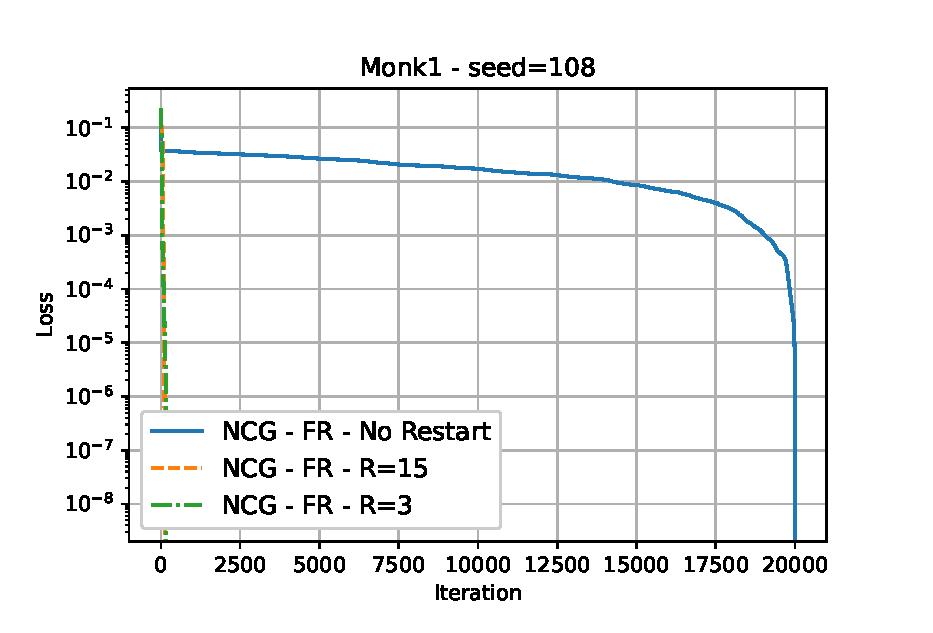
\includegraphics[width=1.1\linewidth]{Images/monk1_fr.eps}
         \caption{FR with no restart, FR with R=15, and FR with R=3.}
         \label{fig:FR_monk_1_non_zoomed}
     \end{subfigure}
     \hfill
     \begin{subfigure}[b]{.497\textwidth}
         \centering
         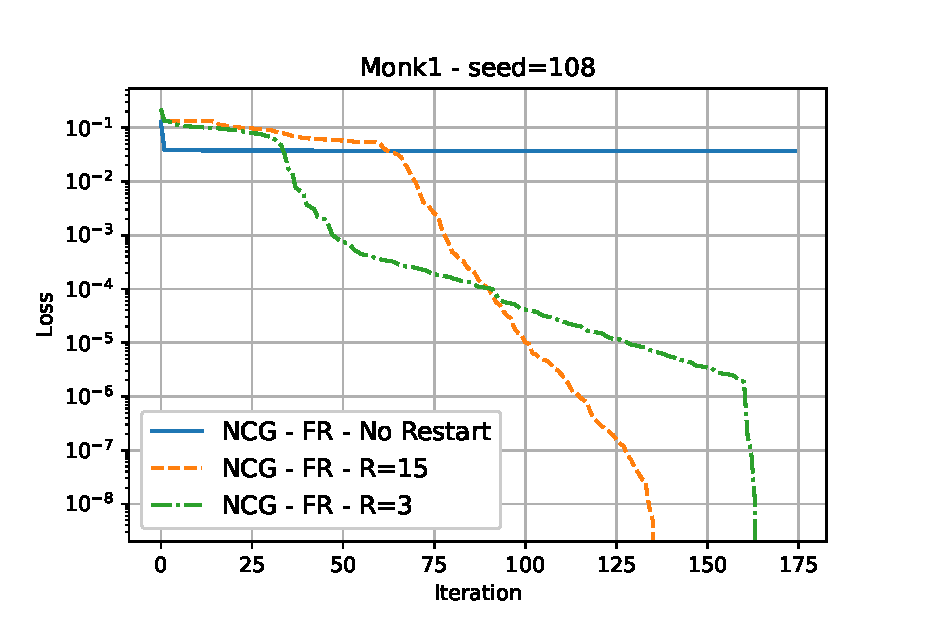
\includegraphics[width=1.1\linewidth]{Images/monk1_fr_zoomed.eps}
         \caption{Zoomed version of Fig.\ref{fig:FR_monk_1_non_zoomed}.}
         \label{fig:FR_monk_1_zoomed}
     \end{subfigure}
     \caption{Loss with respect to the minima. NCG - FR applied to $Monk1$, with three different restarts. The details of these experiments (No restart - \#1, R=15 - \#2, R=3 - \#3) are in Tab.\ref{tab:f1_behavior} and in Tab.\ref{tab:ls_statistics}.}
     \label{fig:FR_monk_1}
\end{figure}

%\cgv{CONVERGENT RATE: R=3 lineare con qualche picco superlineare all'inizio e alla fine (non arriva mai a 1.5). Idem per R=15, sembra abbia più picchi superlineari (ma sempre poco sopra 1). R=0 lineare con un'unica punta superlineare alla fine. I due FR con restart convergono ad un minimo della stessa qualità, quindi possiamo dire che in questo caso R=15 è meglio perché converge con meno iterazioni}\\
%Moreover, we can observe how the method behaves in terms of local convergence. From Fig~\ref{fig:FR_monk_1} we can state that, thanks to the restart, the method can reach the superlinear rate of convergence in both experiments 2 and 3. Moreover, the experiment 2, with restart equal to 15, can reach almost a quadratic rate of convergence (as expected from the theory if the restart is chosen correctly ). Finally, if we compare experiments 2 and 3 in terms of time, with restart 15 and 3, efficiency improvement is significant ($2.30s$ vs $4.07$).

%As can be seen from Tab~\ref{tab:f1_behavior}, only $ls\_max\_iter = 100$ has been tested as line search max iteration parameter. This gave excellent results and has been maintained for all experiments performed with the FR method. In fact, by looking to the summary table~\ref{tab:ls_statistics} for the line search statistics, we can see how the line search hit rate is very high for experiments 1,2 and 3. The behavior with different $ls\_max\_iter$ values will be shown later.


\subsubsection{PR and PR+ methods}
\begin{table}[H]
\small
%\footnotesize
    \centering
    \begin{tabular}{ |c|c|c|c|c|c|c|c|c|c|c|}
    \hline
     \multicolumn{11}{|c|}{\textbf{PR and PR+ analysis results}} \\
      \hline
       \textbf{\#} & \textbf{\textit{f}} & \textbf{Seed} & \textbf{Method} & $\mathbf{c_1}$ & $\mathbf{c_2}$ & \textbf{Ls Max Iter.} & $\mathbf{\textit{\textbf{f}}\,^*}$ & $\mathbf{\norm{\mathbf{g}_k}}$ & \textbf{Conv. Iter.} & \textbf{Time (s)}\\
     \hline
      4 & $Monk1$ & 108 & NCG PR & 1e-4 & 0.1 & 100 & 2.63e-2 & 6.98e-6 & 126 & 1.83\\
      \hline
      5 & $Monk1$ & 108 & NCG PR+ & 1e-4 & 0.1 & 100 & 2.63e-2 & 9.19e-6 & 103 & 1.09\\
      \hline
      6 & $Monk1$ & 206 & NCG PR & 1e-4 & 0.3 & 100 & 2.64e-2 & 5.39e-6 & 305 & 3.93\\
      \hline
      7 & $Monk1$ & 206 & NCG PR+ & 1e-4 & 0.3 & 100 & 2.64e-2 & 8.40e-6 & 191 & 2.08\\
      \hline
    \end{tabular}
    \caption{Results of the experiments with the NCG - PR/PR+.}
    \label{tab:pr_behavior}
\end{table}

Even if this section it's not dedicated to the study of methods efficiency from the same starting point, for the PR and PR+ we decided to analyze them with the same seed used for the FR method in order to check if these two methods behave better than FR. In fact, experiments 4 and 5, shown in Tab.~\ref{tab:pr_behavior}, reveal the efficiency of the PR/PR+ formulas, which reach a minimum of the same quality of the one found by the FR with restart, in fewer iterations. Moreover, from both figures Fig.~\ref{fig:monk1_pr_pr+_108} and Fig.~\ref{fig:monk1_pr_pr+_206}, we can see that the PR+ approaches the same minimum of PR faster.
This is very interesting because it points out that the presence of beta negative in some iterations may affect the convergence efficiency of the method.
\begin{figure}[H]
     \centering
     \begin{subfigure}[b]{.497\textwidth}
         \centering
         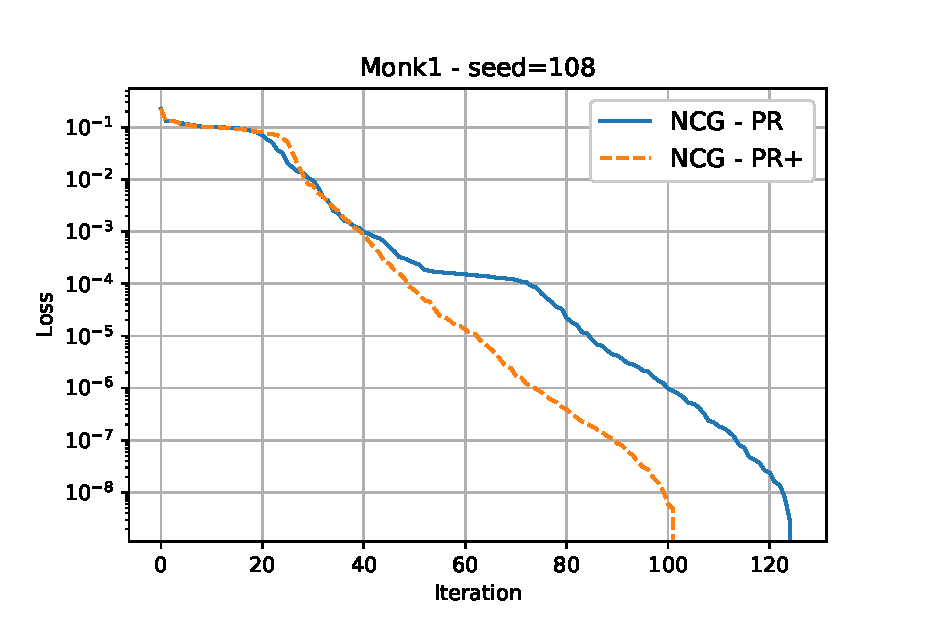
\includegraphics[width=1.1\linewidth]{Images/monk1_pr_pr+_1.eps}
         \caption{PR and PR+, respectively experiments \#4 and \#5.}
         \label{fig:monk1_pr_pr+_108}
     \end{subfigure}
     \hfill
     \begin{subfigure}[b]{.497\textwidth}
         \centering
         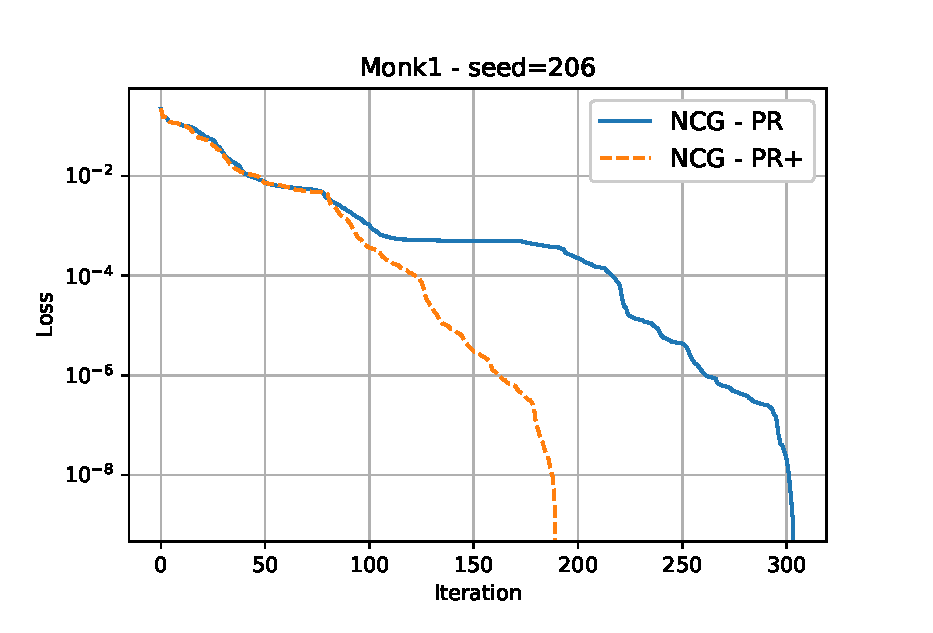
\includegraphics[width=1.1\linewidth]{Images/monk1_pr_pr+_2.eps}
         \caption{PR and PR+, respectively experiments \#6 and \#7.}
         \label{fig:monk1_pr_pr+_206}
     \end{subfigure}
    \caption{Loss with respect to the minima. NCG - PR and NCG - PR+ applied to $Monk1$. Details are in Tab.\ref{tab:pr_behavior} and in Tab.\ref{tab:ls_statistics}.}
    \label{fig:monk1_pr_pr+}
\end{figure}

%Afterward, in some experiments, we have observed how important is the max number of iterations of the line search to almost always find an alpha that respects the conditions of strong Wolfe at each iteration of the optimization process. In Fig~\ref{fig:monk2_pr_pr+_189_line_10} are shown the experiments 8 and 9, where the $ls\_max\_iter$ is equal to 10. It can be observed that, at the beginning of the curve, the rate of convergence is quadratic, but after the rate becomes sub-linear. In this last range, the line search starts to fail. Indeed, from Tab.~\ref{tab:ls_statistics}, we can see that the hit rate drops to 11\% and 8\%, respectively, to experiments 8 and 9. Moreover, the optimization process ends for maximum number of iterations, without reaching the threshold on the value of the loss or gradient norm, in any case both are converging to a local minima because the gradient norm is in the order of $1\mathrm{e}{-6}$. Instead, if we use the same objective function, optimizer configuration and starting point but with $ls\_max\_iter$ equal to 100, the behavior changes drastically. This analysis is related to experiment 10 and 11, where the rate of convergence is quadratic in the first 45 iterations, and linear up to the converge. In those experiments the hit rate of the line search is 97\%. These and other details of those experiments can be found in Tab.~\ref{tab:pr_behavior} and Tab.~\ref{tab:ls_statistics}. 

Regarding the convergencerate, all the methods seem to have a linear trend, with a few superlinear peaks (see Fig.~\ref{fig:monk1_pr_pr+}). 

In addition, we have verified that the use of the restart parameter was not very useful, thanks to the nature of the beta formula that performs an automatic restart when bad directions are reached, as said from the theory. For this reason no analysis has been reported when this parameter changes. Therefore, also the PR/PR+ methods behave as expected from the theoretical analysis made.

%It is interesting to note that if the line search fails a lot, then the optimization process will requires more time spent during the line search phase compared to the total time. For example if we consider experiment 9 with PR+ and $ls\_max\_iter = 10$, it needs $28.26s$ to complete the whole optimization process and $19.73s$ are only for the line search, in fact the hit rate is $8\%$. Instead the same with the same objective function and same setting for the optimization process, experiment 11, the total time is $4.64$ and only 

\subsubsection{HS and HS+ methods}
\begin{table}[H]
\small
%\footnotesize
    \centering
    \begin{tabular}{ |c|c|c|c|c|c|c|c|c|c|c|}
    \hline
     \multicolumn{11}{|c|}{\textbf{HS and HS+ analysis results}} \\
      \hline
       \textbf{\#} & \textbf{\textit{f}} & \textbf{Seed} & \textbf{Method} & $\mathbf{c_1}$ & $\mathbf{c_2}$ & \textbf{Ls Max Iter.} & $\mathbf{\textit{\textbf{f}}\,^*}$ & $\mathbf{\norm{\mathbf{g}_k}}$ & \textbf{Conv. Iter.} & \textbf{Time (s)}\\
     \hline
      8 & $Monk3$ & 353 & NCG HS & 1e-4 & 0.1 & 100 & 3.53e-2 & 9.31e-8 & 281 & 3.58\\
      \hline
      9 & $Monk3$ & 353 & NCG HS+ & 1e-4 & 0.1 & 100 & 3.53e-2 & 9.06e-8 & 331 & 4.62\\
      \hline
    \end{tabular}
    \caption{Results of the experiments with the NCG - HS/HS+.}
    \label{tab:hs_behavior}
\end{table}

General tests have shown that the behavior of HS/HS+ behave quite similar to the PR/PR+. For this reason we are not going to examine it in details and we leave the comparison analysis from the same starting point in the next section. We decided to present here an experiment on the $Monk3$ objective function, with the $\mathbf{w}_0$ generated by seed 353 and compare the HS and the HS+ methods. We can observe that the methods reach a minimum of the same quality ($f^* = 3.53\mathrm{e}{-2}$), but HS, in this case, converges in fewer iterations (see Fig.~\ref{fig:monk3_hs_hs+}).
As expected, the convergence rate is linear, superlinear in very few iterations.
This concludes the analysis and validation of NCG methods and shows that beta negative is not always a bad thing in terms of efficiency. Attention must be paid to the choice of method according to the objective function that is taken in the analysis. 
\begin{figure}[H]
         \centering
         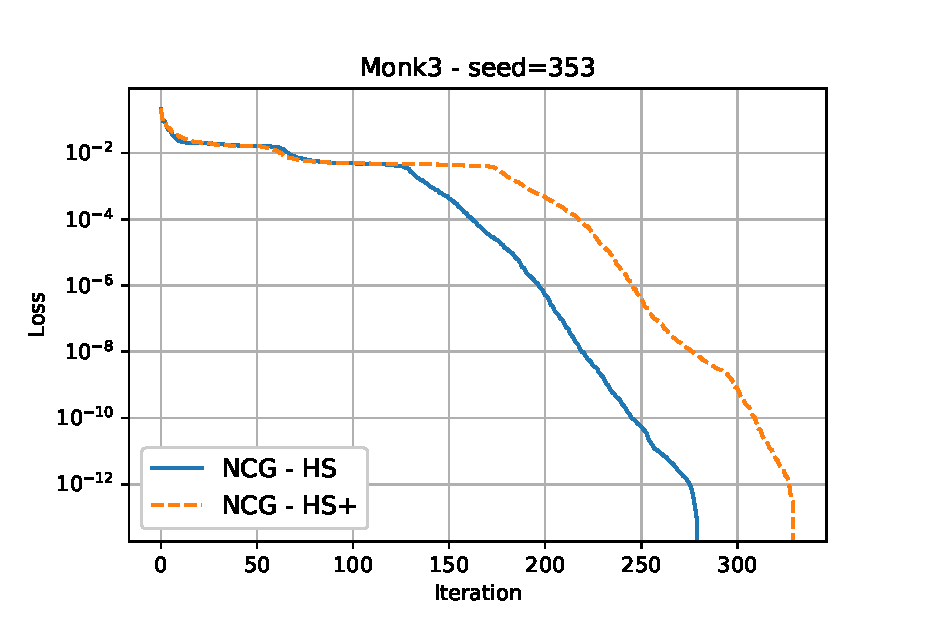
\includegraphics[scale = 0.6]{Images/monk3_hs_hs+.eps}
         \caption{Loss with respect to the minima. NCG - PR and NCG - PR+, respectively experiments \#8 and \#9, applied to $Monk3$. Details are in Tab.\ref{tab:hs_behavior} and in Tab.\ref{tab:ls_statistics}.}
    \label{fig:monk3_hs_hs+}
\end{figure}


\subsubsection{L-BFGS method}
\begin{table}[H]
\small
%\footnotesize
    \centering
    \begin{tabular}{ |c|c|c|c|c|c|c|c|c|c|c|}
    \hline
     \multicolumn{11}{|c|}{\textbf{L-BFGS analysis results}} \\
      \hline
       \textbf{\#} & \textbf{\textit{f}} & \textbf{Seed} & \textbf{m} & $\mathbf{c_1}$ & $\mathbf{c_2}$ & \textbf{Ls Max Iter.} & $\mathbf{\textit{\textbf{f}}\,^*}$ & $\mathbf{\norm{\mathbf{g}_k}}$ & \textbf{Conv. Iter.} & \textbf{Time (s)}\\
     \hline
      10 & $Monk2$ & 987 & 3 & 1e-4 & 0.9 & 100 & 2.82e-2 & 2.80e-5 & 123 & 0.32\\
      \hline
      11 & $Monk2$ & 987 & 30 & 1e-4 & 0.9 & 100 & 2.82e-2 & 2.91e-5 &  74 & 0.58\\
      \hline
    \end{tabular}
    \caption{Results of the experiments with the L-BFGS.}
    \label{tab:lbfgs_behavior}
\end{table}


From the theory in Sec.~\ref{convergence_qn}, we saw that the L-BFGS does not converge with certainty to a stationary point in our case. Indeed, this property strongly depends on the starting point. However, if the algorithm at some point enters and stays in a compact region where the function is smooth strongly convex, then it converges. Moreover, during the optimization process, we have checked that the curvature condition in Eq.~\ref{curvature_condition} is epsilon respected at each iteration: $\mathbf{s}_k^T\mathbf{y}_k > 1\mathrm{e}{-8}$. Indeed, a bad starting point and the wrong parameters would bring to a negative curvature condition, and at the end of the process. This behavior was widely seen during our experiments.
We have also noticed that the method is more unstable numerically in the convergence process then the NCG. In fact, when it reach the gradient norm of the order of $1\mathrm{e}{-6}$ the curvature condition becomes negative.

We reported in Tab.~\ref{tab:lbfgs_behavior} only two experiment (10 and 11) with different value of $m$ parameter, and from Fig.~\ref{fig:monk3_lbfgs} we can see that the algorithm is able to converges in these configurations. The convergence rate for both the experiments is only linear, with some superlinear peaks. Regarding the line search, as we expect from the theory, an $\alpha=1$ is almost always accepted. Indeed, how we can see from Tab.~\ref{tab:ls_statistics}, the L-BFGS performs very few line search iterations compared to other methods, and this is a confirmation of the above. Finally, from Fig.~\ref{fig:monk3_lbfgs} we can see how the convergence speed of the algorithm varies as $m$ varies. Indeed, the experiment wit $m=30$ converges faster than the one with $m=3$, highlighting that, if more curvature information is stored, fewer iterations are needed for the algorithm to reach a minimum of the same quality ($f^* = 2.82\mathrm{e}{-2}$).


\begin{figure}[H]
\footnotesize
    \centering
    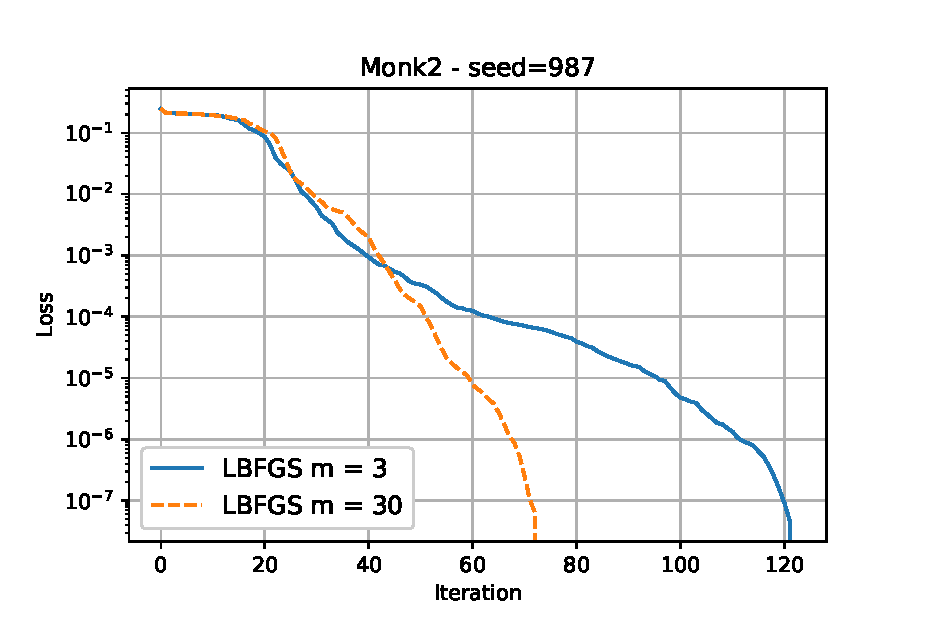
\includegraphics[scale = 0.6]{Images/m2-987_lbfgs.eps}
    \caption{Loss with respect to the minima. L-BFGS experiments \#10 ( =3) and \#11 (m=30), on $Monk2$. Details in Tab.\ref{tab:lbfgs_behavior} and in Tab.\ref{tab:ls_statistics}.}
    \label{fig:monk3_lbfgs}
\end{figure}



\subsection{Methods comparisons}\label{sec:method_comparisons}
From the analysis carried out in the previous section, we decided to exclude the PR and HS methods from the comparison, because with our objective functions and the starting points chosen in this comparisons, we never achieved better results than their modified counterparts. In addition, this allows us to better visualize and compare methods, being less. To study the efficiency of the various methods we have selected a starting point for each objective function, through a seed. Then we have chosen the tolerances for all methods, so that we can compare the behavior towards a certain loss value. After that we compared the result of the optimization process for the following methods: FR with restart, PR+, HS+ and L-BFGS. The following table contains the seed and the tolerance used for each objective function. $ls\_\max\_iter = 100$ has been used for line search given the excellent results of the previous studies.
\begin{table}[H]
\small
    \centering
    \begin{tabular}{|c|c|c|c|c|}
        \hline
        \multicolumn{5}{|c|}{\textbf{Stop criteria and seed}} \\
        \hline
        \textit{\textbf{f}}   & \textbf{seed} &\textbf{ng\_eps} & \textbf{l\_eps} & \textbf{max\_iter} \\
        \hline
        $Monk1$ & 6 & $3\mathrm{e}{-5}$ & $1\mathrm{e}{-6}$ & 1000 \\
        \hline
        $Monk2$ & 189 & $3\mathrm{e}{-5}$ & $1\mathrm{e}{-6}$ & 1000 \\
        \hline
        $Monk3$ & 783 & $10\mathrm{e}{-6}$ & $1\mathrm{e}{-6}$ & 1000 \\
        \hline
    \end{tabular}
    \caption{Stop criteria and seeds used for the methods comparison. }
    \label{tab:monk_stop_criteria_method_comparison}
\end{table}
As regards the analysis of the convergence rate, we used both the logarithm scale plots, as explained in the previous section, and also those related to the rate of convergence $p$ estimation. A sequence $\{f_k\}$ that converges to $f^*$ is said to have rate of convergence $p$ if
$$ \lim_{k \rightarrow \inf} \frac{\lvert f_{k+1}-f^* \rvert}{\lvert f_{k}-f^* \rvert^p} = R >0,$$
and from that $p$ can be estimate with the following formula,
$$ p = \lim_{k \rightarrow \inf} \frac{\log\lvert f_{k+1}-f^* \rvert - \log R}{\log\lvert f_{k}-f^* \rvert^p} \approx \lim_{k \rightarrow \inf} \frac{\log\lvert f_{k+1}-f^* \rvert}{\log\lvert f_{k}-f^* \rvert^p} $$
The convergence rate is linear if $p=1$, $p>1$ is superlinear and $p=2$ for a quadratic rate.
%The results are shown in the Tab.~\ref{tab:method_comparisons} and the line search statistics can be found in Tab.~\ref{tab:method_comparisons_ls}. 


%We can see from Tab.~\ref{tab:method_comparisons} that all methods converge very close to a local minimum and all stops because of the loss threshold. In fact, the gradient norm and the loss value have an order of $\approx 1\mathrm{e}{-12}$ and $1\mathrm{e}{-14}$ in all the configuration. From the time comparison we can observe that L-BFGS can use very efficiently the approximation of the hessian to converge quickly to a certain loss value compared to all the others, for example for the $Monk1$ the L-BFGS converge to the threshold loss in only $0.14s$, instead, the other method takes much more (e.g FR method require $1.45s$.
%As for the rate of convergence, the same behaviors have been observed in these configurations as in the section dedicated to the study of individual methods. The superlinear and quadratic convergence can be observed in all the configuration as shown in Fig.~\ref{fig:test1}, \ref{fig:test2} and \ref{fig:test3}, releted to $Monk1$, $Monk2$ and $Monk3$.


\subsubsection{Monk1}

All the methods stop because they have reached epsilon optimality on the gradient norm. Tab.~\ref{tab:monk1_method_comparisons} shows the result of the methods for the $Monk1$ objective function. All the algorithms converge to a minimum of the same quality (the values differ at most of 0.22e-2), but the L-BFGS reaches the optimal value in fewer iterations than the others. In this case, the L-BFGS is the most efficient because it has the lowest  $\textit{f}\,^*$, and it is also the fastest (needs only 0.26s to reach the stop condition). The reason is related to the number of iterations carried out in the line search method. Indeed, as can be seen from Tab~\ref{tab:monk1_method_comparisons_ls}, the L-BFGS needs only 20 iterations, because $\alpha = 1$ is almost always accepted (fewer iterations than those of other methods, for example, HS+ requires 507). The convergence rate of all the NCG methods is linear, with some superlinear peaks, instead the L-BFGS is almost always superlinear (see Fig.~\ref{fig:sub2}).

\begin{table}[H]
\small
%\footnotesize
    \centering
    \begin{tabular}{ |c|c|c|c|c|c|c|c|c|c|}
    \hline
     \multicolumn{10}{|c|}{\textbf{Best results on \textit{f}: $Monk1$}} \\
      \hline
       \textbf{\textit{f}} & \textbf{Optimizer} & \textbf{c1} &  \textbf{c2} & \textbf{restart} & \textbf{m} & $\mathbf{\textit{\textbf{f}}\,^*}$ & $\norm{\mathbf{g}_k}$ & \textbf{Conv. Iter.} & \textbf{Time (s)}\\
     \hline
      $Monk1$ & NCG FR & 1e-4 & 0.3  & 3  & -  & 2.92e-2  & 2.24e-5 & 125  & 0.94\\
      \hline
      $Monk1$ & NCG PR+ & 1e-4 & 0.4  & -  & -  & 2.84e-2  & 2.80e-5 & 158  & 0.96\\
      \hline
      $Monk1$ & NCG HS+ & 1e-4 & 0.6  & -  & -  & 2.92e-2  & 2.71e-5 & 91  & 0.75\\
      \hline
      $Monk1$ & L-BFGS & 1e-4 & 0.9  & -  & 30  & 2.70e-2  & 1.98e-5 & 80  & 0.26\\
      \hline
    \end{tabular}
    \caption{Methods comparisons results with the $Monk1$ objective function and the $\mathbf{w}_0$ generated by seed 6.}
    \label{tab:monk1_method_comparisons}
\end{table}

\begin{table}[H]
\small
%\footnotesize
    \centering
    \begin{tabular}{ |c|c|c|c|c|c|c|c|c|c|}
    \hline
     \multicolumn{6}{|c|}{\textbf{Line search statistics of Tab.~\ref{tab:monk1_method_comparisons}}} \\
      \hline
       \textbf{\textit{f}} & \textbf{Optimizer} & \textbf{Ls Max Iter.} &  \textbf{Ls Iter.} & L\textbf{s Hit Rate} & \textbf{Ls Time (s)}\\
     \hline
      $Monk1$ & NCG FR & 100 & 678 & 100\%  & 0.73\\
      \hline
      $Monk1$ & NCG PR+ & 100 & 886 & 100\%  & 0.74\\
      \hline
      $Monk1$ & NCG HS+ & 100 & 507 & 100\%  & 0.56\\
      \hline
      $Monk1$ & L-BFGS & 100 & 20 & 100\%  & 0.05\\
      \hline
    \end{tabular}
    \caption{Results of the line search statistics related to Tab.~\ref{tab:monk1_method_comparisons}}
    \label{tab:monk1_method_comparisons_ls}
\end{table}

\begin{figure}[H]
\centering
\begin{subfigure}{.5\textwidth}
  \centering
  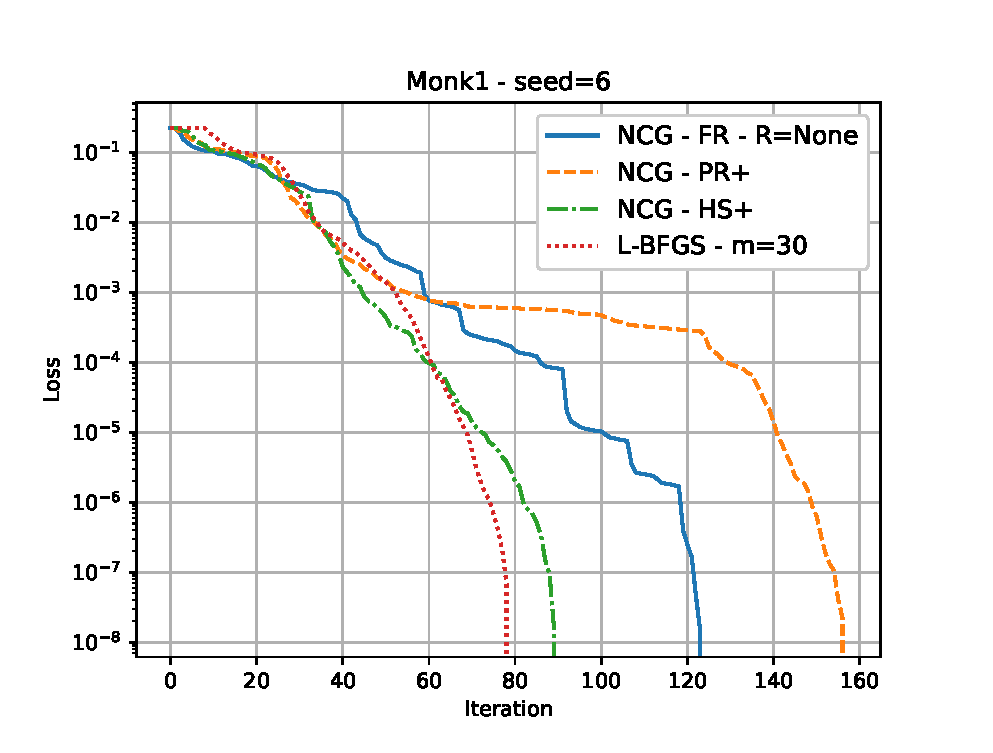
\includegraphics[width=1.1\linewidth]{Images/m1-6_comp.eps}
  \caption{$Monk 1$}
  \label{fig:sub1}
\end{subfigure}%
\begin{subfigure}{.5\textwidth}
  \centering
  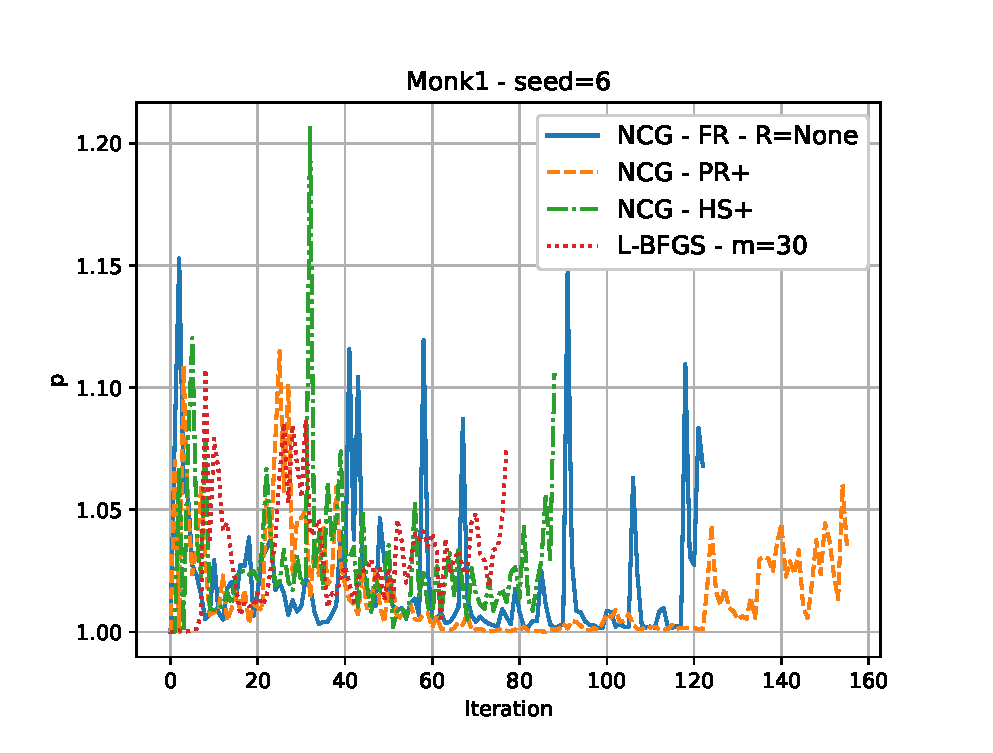
\includegraphics[width=1.1\linewidth]{Images/m1-6_comp_p.eps}
  \caption{$Monk1$ $p$ estimation.}
  \label{fig:sub2}
\end{subfigure}
\caption{Comparisons between methods considering the $Monk1$  objective function and the same starting point generated by seed 6.}
\label{fig:test1}
\end{figure}

\subsubsection{Monk2}
As for $Monk1$, here the same occurs, epsilon optimality is reached on the gradient norm and all the methods converge to a minimum of the same quality (the values differ at most of 0.02e-2), but the L-BFGS reaches the optimal value in fewer iterations than the others (see Tab.~\ref{tab:monk2_method_comparisons}). Moreover, the computational time of the L-BFGS is the smallest. The convergence rate of all the NCG methods is linear, with some superlinear peaks, instead the L-BFGS is almost always superlinear (see Fig.~\ref{fig:sub4})

\begin{table}[H]
\small
%\footnotesize
    \centering
    \begin{tabular}{ |c|c|c|c|c|c|c|c|c|c|}
    \hline
     \multicolumn{10}{|c|}{\textbf{Best results on \textit{f}: $Monk2$}} \\
      \hline
       \textbf{\textit{f}} & \textbf{Optimizer} & \textbf{c1} &  \textbf{c2} & \textbf{restart} & \textbf{m} & $\mathbf{\textit{\textbf{f}}\,^*}$ & $\norm{\mathbf{g}_k}$ & \textbf{Conv. Iter.} & \textbf{Time (s)}\\
     \hline
      $Monk2$ & NCG FR & 1e-4 & 0.3  & 3  & -  & 2.82e-2  & 2.89e-5 & 171  & 1.04 \\
      \hline
      $Monk2$ & NCG PR+ & 1e-4 & 0.1  & -  & -  & 2.82e-2  & 2.60e-5 & 138  & 0.91 \\
      \hline
      $Monk2$ & NCG HS+ & 1e-4 & 0.1  & -  & -  & 2.82e-2  & 2.45e-5 & 94  & 0.6 \\
      \hline
      $Monk2$ & L-BFGS & 1e-4 & 0.9  & -  & 20  & 2.84e-2  & 1.62e-5 & 75  & 0.3\\
      \hline
    \end{tabular}
    \caption{Method comparison results with the $Monk2$ obj. function and the $\mathbf{w}_0$ generated by seed 189.}
    \label{tab:monk2_method_comparisons}
\end{table}

\begin{table}[H]
\small
%\footnotesize
    \centering
    \begin{tabular}{ |c|c|c|c|c|c|c|c|c|c|}
    \hline
     \multicolumn{6}{|c|}{\textbf{Line search statistics of Tab.~\ref{tab:monk2_method_comparisons}}} \\
      \hline
       \textbf{\textit{f}} & \textbf{Optimizer} & \textbf{Ls Max Iter.} &  \textbf{Ls Iter.} & L\textbf{s Hit Rate} & \textbf{Ls Time (s)}\\
     \hline
      $Monk2$ & NCG FR & 100 & 889 & 100\%  & 0.8  \\
      \hline
      $Monk2$ & NCG PR+ & 100 & 834 & 100\%  & 0.73\\
      \hline
      $Monk2$ & NCG HS+ & 100 & 555 & 100\%  & 0.48 \\
      \hline
      $Monk2$ & L-BFGS & 100 & 1 & 100\%  & 0.05 \\
      \hline
    \end{tabular}
    \caption{Results of the line search statistics related to Tab.~\ref{tab:monk2_method_comparisons}}
    \label{tab:monk2_method_comparisons_ls}
\end{table}

\begin{figure}[H]
\centering
\begin{subfigure}{.5\textwidth}
  \centering
  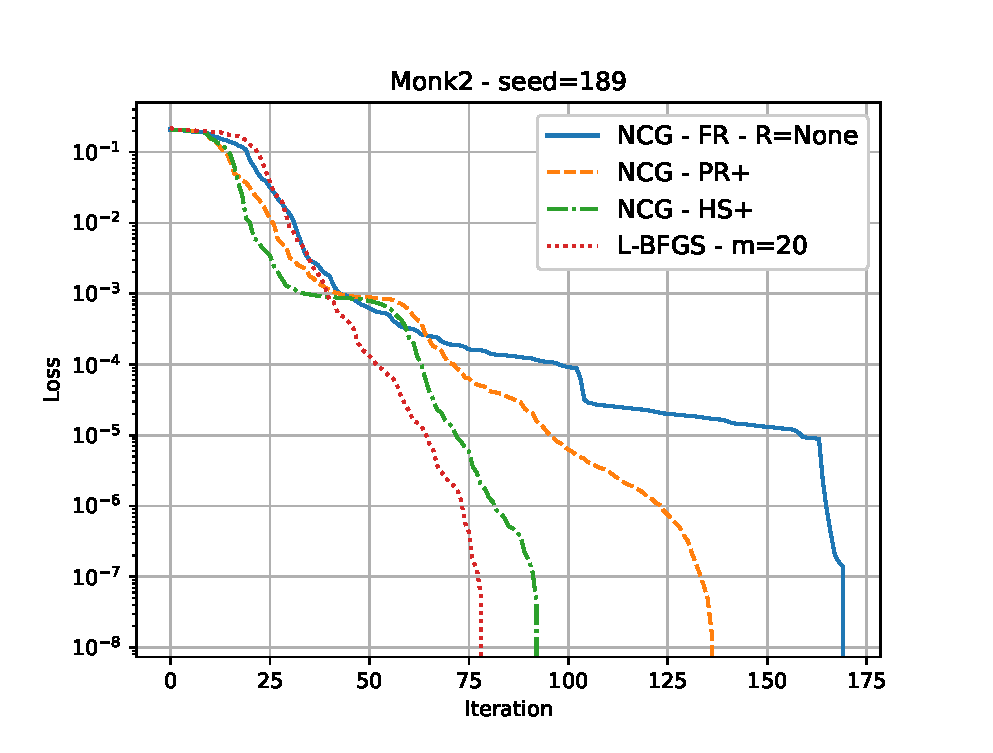
\includegraphics[width=1.1\linewidth]{Images/m2-189_comp.eps}
  \caption{$Monk2$}
  \label{fig:sub3}
\end{subfigure}%
\begin{subfigure}{.5\textwidth}
  \centering
  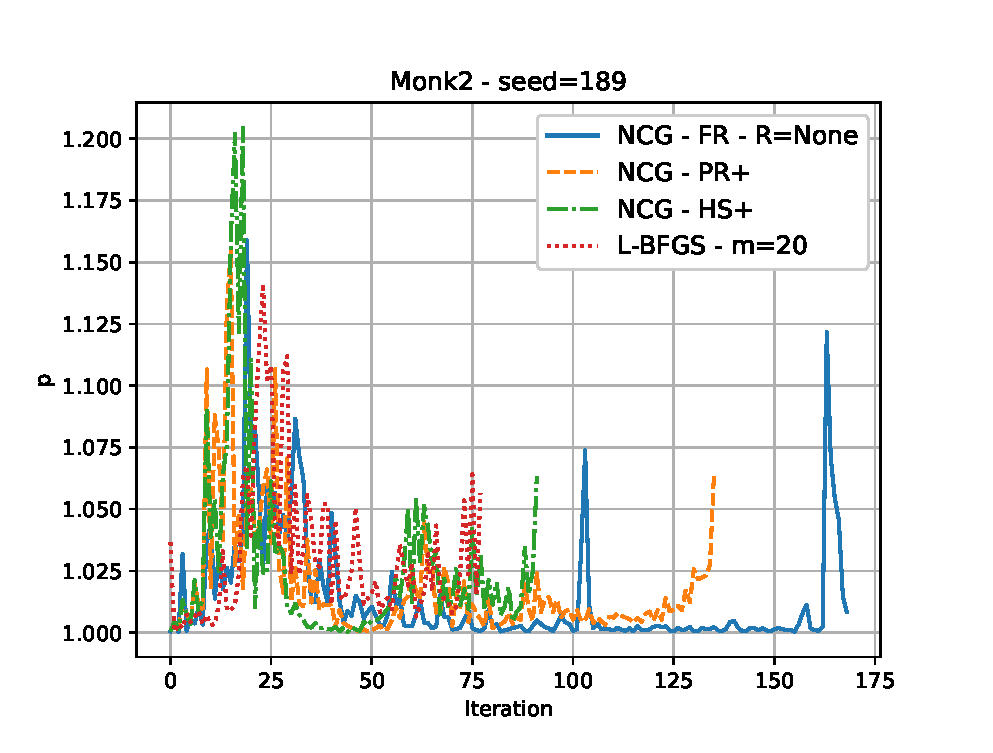
\includegraphics[width=1.1\linewidth]{Images/m2-189_comp_p.eps}
  \caption{$Monk2$ $p$ estimation.}
  \label{fig:sub4}
\end{subfigure}
\caption{Comparisons between methods considering the $Monk2$  objective function and the same starting point generated by seed 189.}
\label{fig:test2}
\end{figure}

\subsubsection{Monk3}

Finally, for $Monk3$ objective function, the optimal minimum reached by the methods is of the same quality (the values differ at most of 0.83e-2, see Tab.~\ref{tab:monk3_method_comparisons}). Moreover, L-BFGS reaches the lowest $\textit{f}\,^*$ value in fewer iterations than the others methods. In addition, the computational time of the L-BFGS is the smallest. The convergence rate of all the methods is linear, with some superlinear peaks (see Fig.~\ref{fig:sub6}).

\begin{table}[H]
\small
%\footnotesize
    \centering
    \begin{tabular}{ |c|c|c|c|c|c|c|c|c|c|}
    \hline
     \multicolumn{10}{|c|}{\textbf{Best results on \textit{f}: $Monk3$}} \\
      \hline
       \textbf{\textit{f}} & \textbf{Optimizer} & \textbf{c1} &  \textbf{c2} & \textbf{restart} & \textbf{m} & $\mathbf{\textit{\textbf{f}}\,^*}$ & $\norm{\mathbf{g}_k}$ & \textbf{Conv. Iter.} & \textbf{Time (s)}\\
     \hline
      $Monk3$ & NCG FR & 1e-4 & 0.1  & 6  & -  & 3.84e-2  & 6.51e-6 & 450  & 2.22 \\
      \hline
      $Monk3$ & NCG PR+ & 1e-4 & 0.1  & -  & -  & 3.58e-2  & 9.43e-6 & 235  & 1.25 \\
      \hline
      $Monk3$ & NCG HS+ & 1e-4 & 0.3  & -  & -  & 3.84e-2  & 7.16e-6 & 401  & 1.94 \\
      \hline
      $Monk3$ & L-BFGS & 1e-4 & 0.9  & -  & 30  & 3.01e-2  & 5.32e-6 & 115  & 0.49\\
      \hline
    \end{tabular}
    \caption{Method comparison results with the $Monk3$ obj. function and the $\mathbf{w}_0$ generated by seed 783.}
    \label{tab:monk3_method_comparisons}
\end{table}

\begin{table}[H]
\small
%\footnotesize
    \centering
    \begin{tabular}{ |c|c|c|c|c|c|c|c|c|c|}
    \hline
     \multicolumn{6}{|c|}{\textbf{Line search statistics of Tab.~\ref{tab:monk3_method_comparisons}}} \\
      \hline
       \textbf{\textit{f}} & \textbf{Optimizer} & \textbf{Ls Max Iter.} &  \textbf{Ls Iter.} & L\textbf{s Hit Rate} & \textbf{Ls Time (s)}\\
     \hline
      $Monk3$ & NCG FR & 100 & 2490 & 100\%  & 1.74 \\
      \hline
      $Monk3$ & NCG PR+ & 100 & 1249 & 100\%  & 0.98 \\
      \hline
      $Monk3$ & NCG HS+ & 100 & 2004 & 100\%  & 1.47\\
      \hline
      $Monk3$ & L-BFGS & 100 & 12 & 100\%  & 0.07 \\
      \hline
    \end{tabular}
    \caption{Results of the line search statistics related to Tab.~\ref{tab:monk3_method_comparisons}}
    \label{tab:monk3_method_comparisons_ls}
\end{table}

\begin{figure}[H]
\centering
\begin{subfigure}{.5\textwidth}
  \centering
  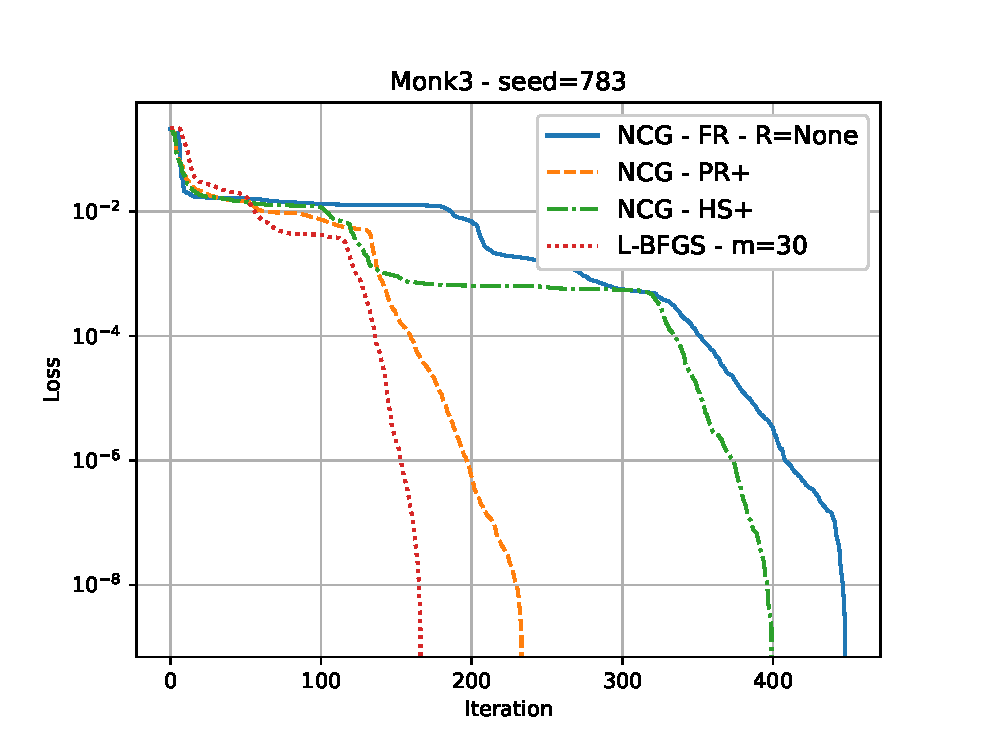
\includegraphics[width=1.1\linewidth]{Images/m3-783_comp.eps}
  \caption{$Monk3$}
  \label{fig:sub5}
\end{subfigure}%
\begin{subfigure}{.5\textwidth}
  \centering
  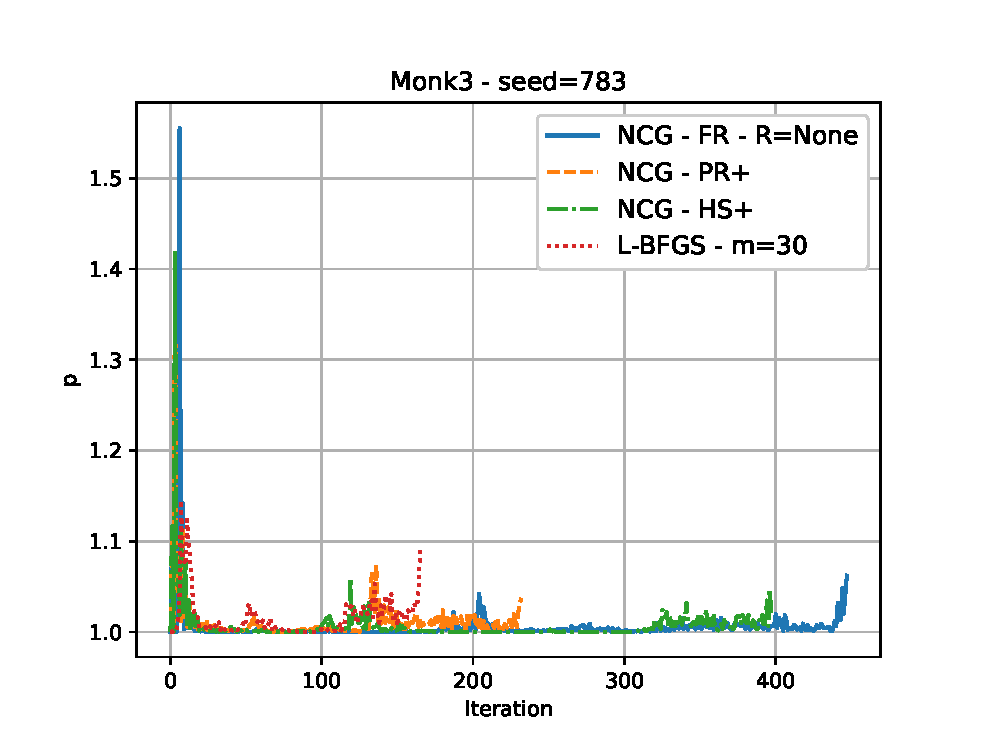
\includegraphics[width=1.1\linewidth]{Images/m3-783_comp_p.eps}
  \caption{$Monk3$ $p$ estimation.}
  \label{fig:sub6}
\end{subfigure}
\caption{Comparisons between methods considering the $Monk3$  objective function and the same starting point generated by seed 783.}\label{fig:test3}
\end{figure}








\section{Conclusions}
\label{sec:conclusions}
In this work, we have presented some methods that make use of more information than classic algorithms such as the nonlinear conjugate gradient and the L-BFGS. Indeed, as a general result, we have noticed that L-BFGS can obtain equal or better results than all the other methods presented here, thanks to the fact that more information is added to generate a descent direction. 
\bibliography{references} 

%\newpage
\begin{appendices}

\end{appendices}


\end{document}
